\chapter{Estimating the luminous region position}\label{chap:beamline}
%\textit{Definition of luminous region, its importance in Alignment and Calibration, luminosity and other stuff}
%\epigraph{Oṃ bhūr buvaḥ svaḥ | tat savitur vareṇyaṃ | bhargo devasya dhīmahi | dhiyo yo naḥ pracodayāt}{Bhagavad Gita, X 15}
The luminous region is defined as the region where the two beams of particles collide, as depicted in Figure \ref{fig:luminous-region}. This region corresponds to the area where the primary vertices of these collisions are formed.



\begin{figure}
    \centering
    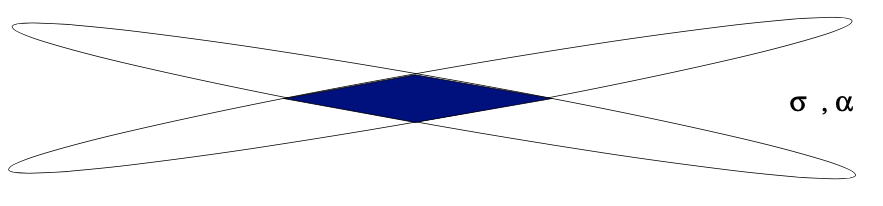
\includegraphics[width=\textwidth]{figures/luminous_region.png}
    \caption{Luminous regions (blue), given the overlap of two bunches}
    \label{fig:luminous-region}
\end{figure}

%\begin{figure}
%    \centering
%    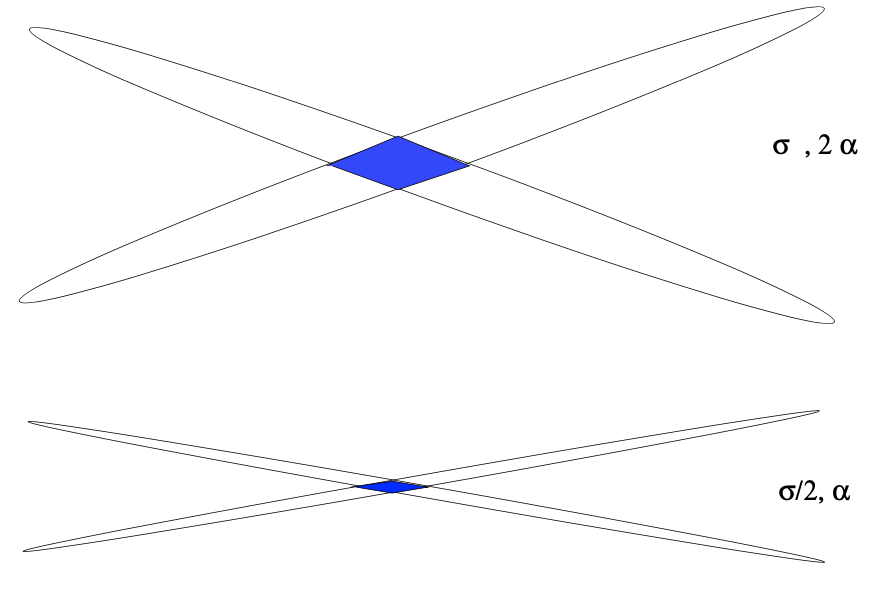
\includegraphics[width=\textwidth]{figures/luminous_region_var.png}
%    \caption{Luminous regions (blue), given the overlap of two bunches with different parameters (width \sigma and crossing angle \alpha) with respect to Figure \ref{fig:luminous-region}}
%    \label{fig:luminous-region-var}
%\end{figure}


Understanding the position of the luminous region is critical for two main reasons:
\begin{itemize}
\item Luminosity Estimation Correction: The luminosity of an experiment is closely tied to the position of the luminous region position. If the luminosity estimate is based on an incorrect luminous region position, the resulting measurements will be skewed. To provide accurate online luminosity estimates, a method is needed to correct for errors in the luminous region position. This implies implementing a data point that continuously monitors the real-time luminous region position to adjust the luminosity calculation accordingly.
\item Track Reconstruction Algorithms: The current algorithms for track reconstruction has relied until 2024 on a predefined, ``hardcoded" position of the luminous region. If this position is not updated accurately, the precision of the track reconstruction can be compromised. A real-time estimation of the luminous region position can enhance the efficiency of track reconstruction.
\end{itemize}

As already stated, both HLT$1$ and HLT$2$ PVs reconstruction algorithms use the luminous region position as an input. Until 2023, the collaboration relied for this information on an iterative track fitting procedure, that computed PVs at HLT$1$ level. The tracks fits were executed in an iterative way until a convergence was reached, making the procedure computationally expensive. Starting from the end of 2023, a YML configuration file named ``InteractionRegion" was created, with the intent of comprehending the luminous region information. This file was manually updated when necessary. In February 2024, the LHCb developed ``BeamSpot Monitor", a tool used for the automatically update of the ``InteractionRegion" configuration file.  This tool operates in the Alignment \& Calibration phase of the online trigger, accumulating statistics and booking histograms of the reconstructed PVs. Once the histograms are available, the mean and covariance are calculated, providing an estimation of the luminous region position to both HLT$1$ and HLT$2$. 

In this chapter, we explore an innovative approach for determining the luminous region position in real-time without relying on traditional track reconstruction algorithms. This approach make use of the cluster counters described in Section \ref{sec:velo_counters}, hence we leverage the capabilities of the clusters provided by the FPGA in order to improve the efficiency of the experiment data analysis processes. Instead of performing an high-level processing at low rates (such as the method currently used), we rely on the low-level statistics at high rates given by the cluster counting process.

It was already shown in an earlier work\cite{dan}, that the counters described in Section \ref{sec:velo_counters} are sensible to a displacement of the luminous region. An example of this sensibility is depicted in Figure \ref{fig:z_lumi_dependency}, where one can clearly see how the mean of the outer counters per event is slightly different depending on the luminous region position. 

\begin{figure}
    \centering
    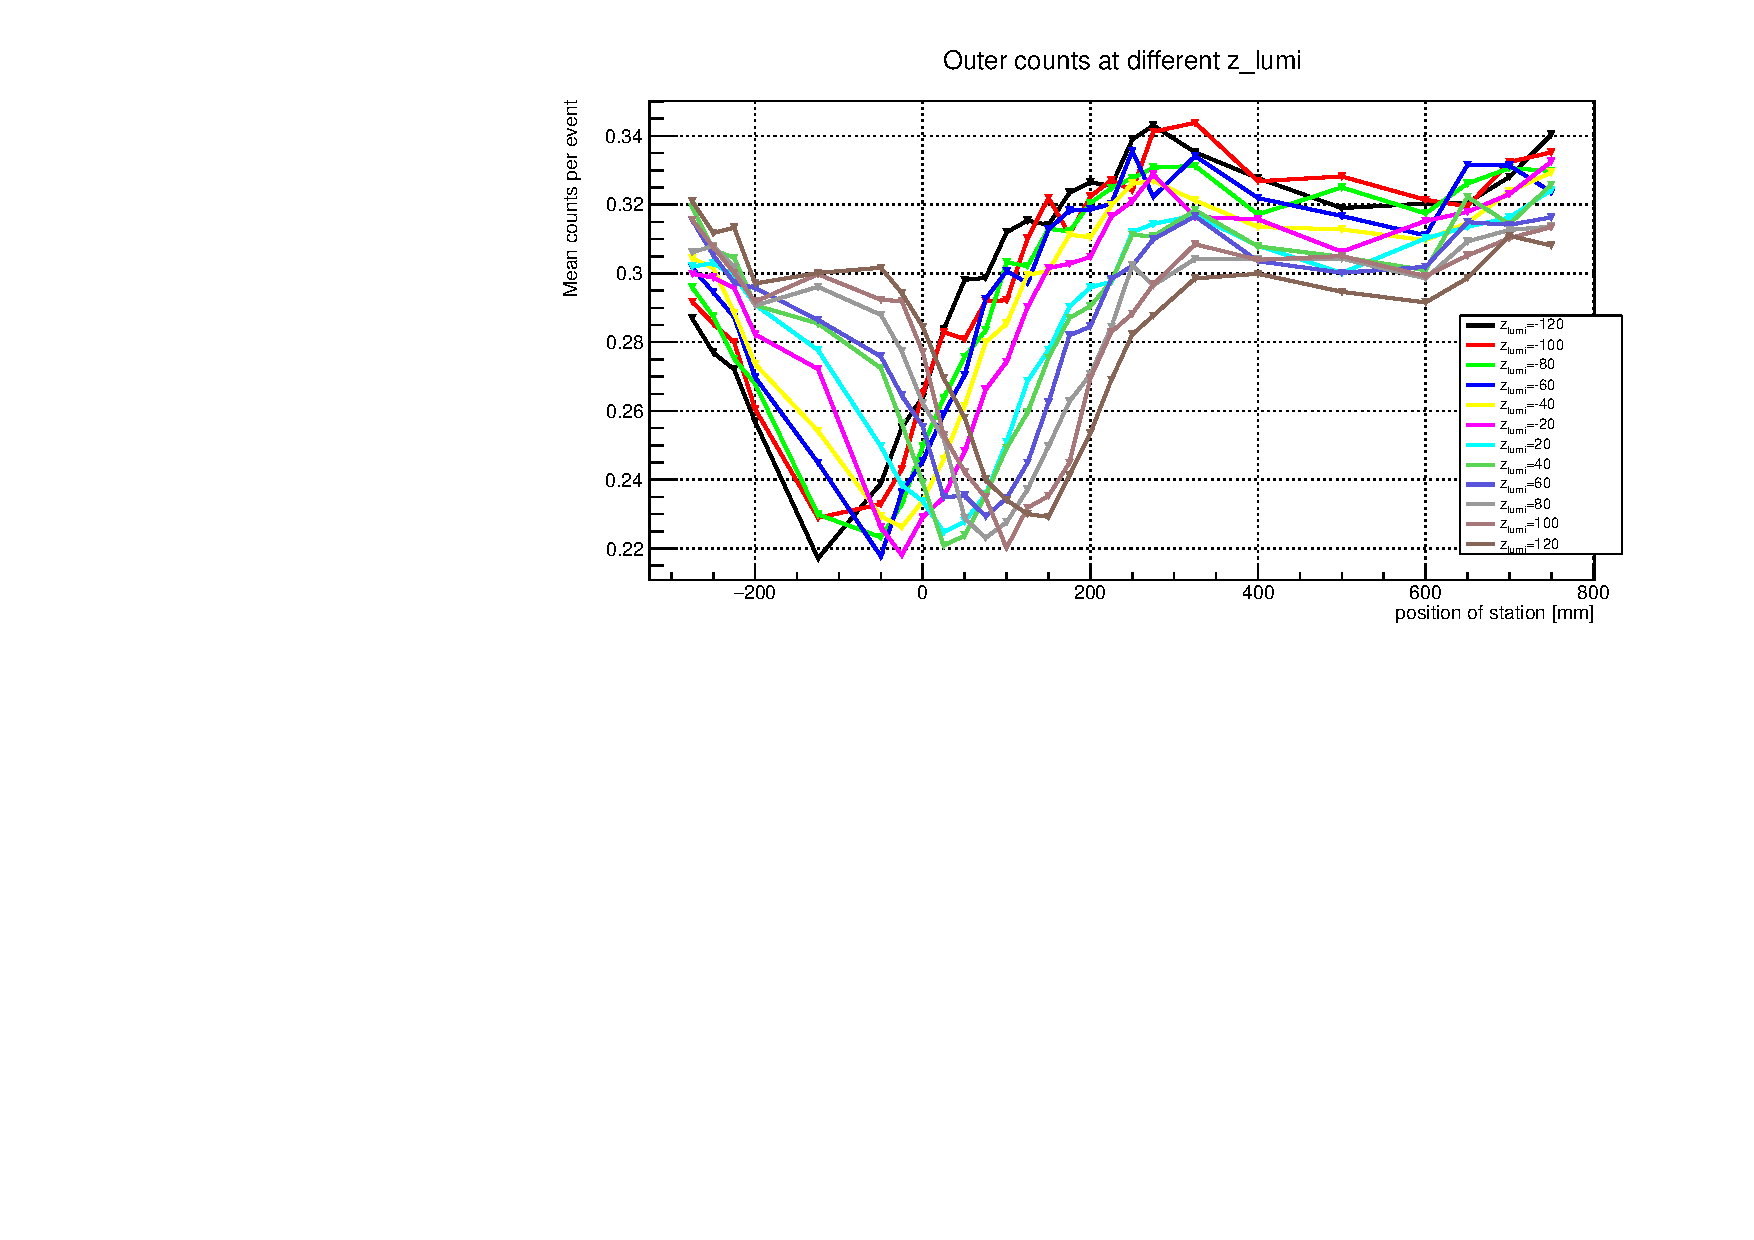
\includegraphics[width=\textwidth]{figures/z_lumi_dependency.pdf}
    \caption{Mean cluster counts per event of the outer counters as a function of the z position of the VELO station on which the counter is implemented. Each different line represents a different simulation on which the luminous region position is displaced as indicated in the legend of the plot.}
    \label{fig:z_lumi_dependency}
\end{figure}

In this chapter, we study a way to combine the 208 implemented counters to give an estimation of the luminous region position in each component x, y, and z. A possibility relies on leveraging the capabilities of a dimensionality reduction technique called Principal Component Analysis, which allows to transform the data in the 208-dimensional space to a space of fewer dimensions. The hope is that the position of the luminous region will be dependent from some of the features extracted with this method. In the next sections, we present this technique, the Monte Carlo simulations used to study the estimators and a calibration and testing on real collision data.

%The Principal Component Analysis is not the only possibility 


\section[The Principal Component Analysis]{The Principal Component Analysis $\bigl($PCA$\bigr)$}\label{sec:PCA}

The Principal Component Analysis (PCA) is a widely used statistical technique for dimensionality reduction, feature extraction, and data compression. It involves transforming a dataset into a new coordinate system with a linear orthogonal transformation designed to maximise the variance along the first principal component (the first coordinate of the transformed system), with the subsequent components containing successively decreasing variance.
An intuition and visualisation of this transformation is given in Figure \ref{fig:pca}.

\begin{figure}
    \centering
    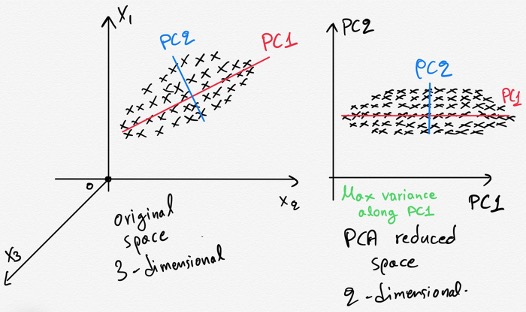
\includegraphics[width=0.8\textwidth]{figures/pca.jpg}
    \caption{Schematic understanding of the Principal Component Analysis: suppose to have a 3 dimensional dataset (left). We can transform this space in a 2 dimensional one (right), with a new basis of two variables given by the two first Principal Components (PC1 and PC2), ordered by the variance captured by the projection of the data on that component.}
    \label{fig:pca}
\end{figure}


Let $\mathbf{X}$ be a $n \times p$ data matrix with column-wise zero empirical mean (the sample mean of each column has been shifted to zero), where $n$ are the number of samples and $p$ the number of features. PCA identifies $l$ principal components (where $l \leq p$) that capture the most variance in the data.

Mathematically, PCA transforms the data by finding a set of size $l$ of $p$-dimensional vectors of weights, or coefficients, $\mathbf{w}_{(k)} = (w_1, \ldots, w_p)_{(k)}$, that map each row vector $\mathbf{x}_{(i)}$ of $\mathbf{X}$ to a new vector of ordered principal component scores $\mathbf{t}_{k} = (t_1, \ldots, t_l)_{(i)}$, defined as:

\begin{equation}
\mathbf{t_{k}}_{(i)} = \mathbf{x}_{(i)} \cdot \mathbf{w}_{(k)} \quad \text{for} \quad i = 1, \ldots, n \quad k = 1, \ldots, l
\end{equation}

The goal is to maximise the variance along each Principal Component (PC), with each coefficient vector $\mathbf{w}$ constrained to be a unit vector. Typically, $l$ is selected to be less than $p$ to reduce dimensionality.


The first PC score $t_{1}$ maximises the variance of the dataset, thus the weight vector $\mathbf{w}_{(1)}$ must satisfy the following condition:

\begin{equation}
\mathbf{w}_{(1)} = \arg \max_{\|\mathbf{w}\| = 1} \left\{ \sum_{i=1}^{n} \left( \mathbf{x}_{(i)} \cdot \mathbf{w} \right)^2 \right\}.\label{argmax}
\end{equation}

Let's break it down to the single pieces: 
\begin{itemize}
    \item $\mathbf{x}_{(i)} \cdot \mathbf{w}$ represents the projection of a data entry $i$ on a direction in the feature space (p-dimensional) described by a vector $ \mathbf{w}$;
    \item $ \sum_{i=1}^{n} \left( \mathbf{x}_{(i)} \cdot \mathbf{w} \right)^2$ is the variance of the projection of the whole dataset on the direction described by the vector $ \mathbf{w}$;
    \item $\|\mathbf{w}\| = 1$ ensures that $\mathbf{w}$ is properly normalised as a unit vector;
    \item the $\arg \max$ operation finds the vector $\mathbf{w}$, such that the projection of the dataset on this vector has the greatest variance, with respect to all the other projections.
\end{itemize}

The condition \ref{argmax} can be rewritten in matrix form as:

\begin{equation}
\mathbf{w}_{(1)} = \arg \max_{\|\mathbf{w}\| = 1} \left\{ \|\mathbf{Xw}\|^2 \right\} = \arg \max_{\|\mathbf{w}\| = 1} \left\{ \mathbf{w}^{\mathsf{T}} \mathbf{X}^{\mathsf{T}} \mathbf{Xw} \right\}.
\end{equation}

Incorporating the normalisation in the analytical form, we get a more straightforward expression:

\begin{equation}
\mathbf{w}_{(1)} = \arg \max \left\{ \frac{\mathbf{w}^{\mathsf{T}} \mathbf{X}^{\mathsf{T}} \mathbf{Xw}}{\mathbf{w}^{\mathsf{T}} \mathbf{w}} \right\}.\label{first_weight}
\end{equation}

The quantity to maximise is recognised as a Rayleigh quotient\cite{horn13}. A positive semidefinite matrix such as $\mathbf{X}^{\mathsf{T}} \mathbf{X}$ has the maximum possible Rayleigh quotient value as its largest eigenvalue, which occurs when $\mathbf{w}$ is the corresponding eigenvector\cite{parlett1998symmetric}.


With $\mathbf{w}_{(1)}$ found, the first PC score of a data vector $\mathbf{x}_{(i)}$ can be calculated as:

\begin{equation}
t_{1(i)} = \mathbf{x}_{(i)} \cdot \mathbf{w}_{(1)}.\label{first_score}
\end{equation}

In order to find subsequent components, the contribution given by $t_{1}$ must be subtracted from the original dataset. This procedure ensures that the subsequent PC focuses on the variance that remains in the data. Iterating the reasoning, the $k$-th PC is found by subtracting the contributions given by the first $k-1$ components. We can hence define a residual matrix $\mathbf{\hat{X}}_{k}$

\begin{equation}
\mathbf{\hat{X}}_{k} = \mathbf{X} - \sum_{s=1}^{k-1} \mathbf{X} \mathbf{w}_{(s)} \mathbf{w}_{(s)}^{\mathsf{T}},\label{dim_red_tran}
\end{equation}
that represents the projection of the data on a subspace orthogonal to the first $k-1$ components.
Creating this matrix $\mathbf{\hat{X}}_{k}$, the problem reduces to the case just discussed, with the solution for $\mathbf{w}_{(k)}$ being the eigenvector with the highest corresponding eigenvalue of the space $\mathbf{\hat{X}}_{k}^\mathsf{T}\mathbf{\hat{X}}_{k}$, since the dataset in the new reduced space is orthogonal to the estimated components described by all the vectors $\mathbf{w}_{(k-1)}$. Furthermore, the eigenvector $\mathbf{w}_{(k)}$ of the residual space $\mathbf{\hat{X}}_{k}$ is the $k$-th  eigenvector of the $\mathbf{X}^{\mathsf{T}} \mathbf{X}$ space since eigenvectors corresponding to distinct eigenvalues are always orthogonal to one another, as stated by the spectral theorem.

This allows us to generalise \eqref{first_score} to a general $k$-th PC score:
\begin{equation}
t_{k(i)} = \mathbf{x}_{(i)} \cdot \mathbf{w}_{(k)}.\label{score}
\end{equation}


%\mathbf{w}_{(k)} = \operatorname{arg\,max}_{\|\mathbf{w}\| = 1} \left\{\|\mathbf{\hat{X}}_{k} \mathbf{w}\|^{2}\right\} = \operatorname{arg\,max} \left\{ \frac{\mathbf{w}^{\mathsf{T}} \mathbf{\hat{X}}_{k}^{\mathsf{T}} \mathbf{\hat{X}}_{k} \mathbf{w}}{\mathbf{w}^{\mathsf{T}} \mathbf{w}} \right\}.



Hence, the weights $\mathbf{w}_{(k)}$ of the PCA are found by diagonalizing the sample covariance matrix $\mathbf{S}$ of the data $\mathbf{X}$, being this defined as:

\begin{equation}
\mathbf{S} =  \frac{1}{n-1} \mathbf{X}^{\mathsf{T}} \mathbf{X} -  \mathbf{\mu_X}^{\mathsf{T}}\mathbf{\mu_X}= \frac{1}{n-1} \mathbf{X}^{\mathsf{T}} \mathbf{X},
%\operatorname {K} _{X_{i}X_{j}}=\operatorname {cov} [X_{i},X_{j}]=\operatorname {E} [(X_{i}-\operatorname {E} [X_{i}])(X_{j}-\operatorname {E} [X_{j}])]
\end{equation}
since $\mathbf{X}$ has column-wise zero empirical mean $\mathbf{\mu_X}=\vec{0}$ by definition. 
In order to find the right order of the PCs, the eigenvectors of $\mathbf{S}$ are then ordered by the magnitude of their eigenvalues, with the largest eigenvalue corresponding to the direction with the most variance in the data (first PC). The (normalised) eigenvalues represent the amount of variance explained by each PC.
Let us summarise the estimation of the weight vectors $\mathbf{w}_{(k)}$ in the Algorithm \ref{alg:weight_PCA}.

\begin{algorithm}
\caption{Principal Component Analysis (PCA)}\label{alg:weight_PCA}
\begin{algorithmic}[1]
    \STATE \textbf{Input:} Dataset \(\mathbf{X}\), with \(n\) samples and \(p\) features, and the desired number of principal components \(l\).

    \STATE \textbf{Step 1:} Compute the covariance matrix \(\mathbf{S}\) of the dataset:
    \begin{equation*}
    \mathbf{S} = \frac{1}{n - 1} \mathbf{X}^{\mathsf{T}} \mathbf{X}.
    \end{equation*}

    \STATE \textbf{Step 2:} Calculate the eigenvectors \(\mathbf{w}_{(k)}\) and eigenvalues \(\lambda_k\) of the covariance matrix \(\mathbf{S}\).

    \STATE \textbf{Step 3:} Sort the eigenvectors \(\mathbf{w}_{(k)}\) by their corresponding eigenvalues in descending order.

    \STATE \textbf{Step 4:} Calculate the first \(l\) principal components for each sample \(\mathbf{x}_{(i)}\):
    \begin{equation*}
    {t_{k}}_{(i)} = \mathbf{x}_{(i)} \cdot \mathbf{w}_{(k)} \quad \text{for} \quad i = 1, \ldots, n \quad k = 1, \ldots, l.
    \end{equation*}
    
    \STATE \textbf{Output:} The principal component scores \(\mathbf{t}\), and the principal component vectors \(\mathbf{w}\).
\end{algorithmic}
\end{algorithm}


The complete principal component decomposition of the data matrix $\mathbf{X}$ can be given in matrix form by:

\begin{equation}
\mathbf{T} = \mathbf{X} \mathbf{W},
\end{equation}

where $\mathbf{W}$ is a $p \times p$ matrix containing the eigenvectors of $\mathbf{S}$.



\section{The Monte Carlo simulations}\label{sec:MC}
To assess the relationship between measured rates on both luminosity and luminous region position, we performed feasibility studies using official LHCb simulations. These simulations allow us to evaluate how variations in luminosity and luminous region parameters impact the detector response.

The LHCb simulation workflow encompasses multiple software applications, each responsible for a specific task. The generation of primary particles from proton-proton collisions is handled by the \textsc{Pythia} package \cite{Sj_strand_2006}, a versatile event generator. Particle decays are simulated through the \textsc{EvtGen} framework \cite{Lange:2001uf}, while the propagation of particles through the detector is modelled with the \textsc{Geant4} toolkit \cite{Agostinelli:2002hh}, which includes a detailed geometric description of all detector components.

All these tasks are managed by the \textsc{Gauss} application \cite{Miglioranzi:1322402}, which integrates the different simulation stages. \textsc{Gauss} also manages various luminosity-related parameters such as pile-up, luminous region position (in \(x, y,\) and \(z\)), its width, beam crossing angle, and luminous region inclination.

The sub-detectors responses to simulated particles are generated by the \textsc{Boole} application, which handles signal digitisation in the same format as the actual experiment's data acquisition system. After digitisation, the simulated data follow the same processing path as real data, passing through the same trigger, reconstruction, and analysis software. The trigger application, known as \textsc{Moore}, includes algorithms for both high-level triggers. 

To investigate the impact of the VELO cluster counters on the luminous region position and luminosity estimations, a software version of the firmware for the luminosity counters was implemented in the \textsc{Moore} framework. This modification allows for the emulation of the hardware functionality, enabling studies of how changes in luminous region parameters affect the counters' readings.

Multiple simulation scenarios were conducted to examine the effects of different settings for instantaneous luminosity and luminous region parameters. All simulations are based on Minimum Bias events, representing generic pp inelastic collisions. They use the LHCb Upgrade I detector simulation with a centre-of-mass energy of $\sqrt{s} = \SI{13.6}{\tera\eV}$ and a bunch spacing of \SI{25}{\nano\second}. Unless specified otherwise, each simulation analysed $10^5$ events. The simulations covered various configurations, writing one file for each configuration:

\begin{enumerate}

    \item[(i)] A scan of the luminous region mean $z$-position from \SI{-120}{\milli\meter} to \SI{120}{\milli\meter} at $\Delta z~=~\SI{20}{\milli\meter}$ steps relative to the LHCb reference frame, with $\nu~=~7.6$, $x~=~\SI{0}{\milli\meter}$, and $y~=~\SI{0}{\milli\meter}$, in MagDown configuration.

    \item[(ii)] A scan of the luminous region mean $y$-position from \SI{-1.5}{\milli\meter} to \SI{1.5}{\milli\meter} at $\Delta~y~=\SI{0.5}{\milli\meter}$ steps relative to the LHCb reference frame, with $\nu~=~7.6$, $x~=~\SI{0}{\milli\meter}$, and $z~=~\SI{0}{\milli\meter}$, in MagDown configuration.

     \item[(iii)] A scan of the luminous region mean $x$-position from \SI{-1.5}{\milli\meter} to \SI{1.5}{\milli\meter} at $\Delta x~=~\SI{0.5}{\milli\meter}$ steps relative to the LHCb reference frame, with $\nu~=~7.6$, $y~=~\SI{0}{\milli\meter}$, and $z~=~\SI{0}{\milli\meter}$, in MagDown configuration.

     \item[(iv)] A scan of event pile-up $\nu$ (i.e. the mean number of PVs per event) from $7.6$ to $35.8$. The mean position of the interaction region was set to $(0.0, 0.0, 0.0)$ mm. Simulations were conducted with both MagDown and MagUp magnet configurations.

\end{enumerate}


The luminous region is an extended 3-dimensional quantity (the distribution of the PVs), hence the value reported on the bullet list above indicate the average position of the PVs. The luminous region is spread for about \SI{30}{\milli\meter} in the $z$ component, while it has a width of \SI{15}{\micro\meter} in both the $x$ and $y$ directions.  

These simulations are used for various purposes. 
\begin{itemize}
\item The simulations in (i), (ii), (iii) are used to construct datasets on which the PCA is performed. As explained in the previous section, the PCA creates a new set of coordinates such that the first coordinate describes the direction of maximal variance of the dataset. If we can construct a dataset in which the only varying component is the luminous region position along one direction and execute the PCA on that dataset, some of the first PCs should be quantities depending on the luminous region position. This procedure is explained in detail in the next section.
\item The simulations in (iv) are used to check for the dependency of the luminous region position estimators to the luminosity. If the luminosity is linear in the counter as explained in Chapter \ref{chap:luminosity}, it follows straightforwardly that the luminosity will also bias the luminous region estimation linearly. This MC simulations are used to verify this behaviour.
\end{itemize}

From each one of the simulation files in (i), (ii), (iii) we produce a tuple containing 212 features:
\begin{itemize}
    \item The event number: it is the index of the tuple indicating the label of the event. It is an integer running from $0$ to $10^5$.
    \item $x$-position [mm]: the $x$ position of the luminous region position reconstructed as the mean of PVs. It is a float number that can assume 7 possible values: $-1.5$, $-1.0$, $-0.5$, $0.0$, $0.5$, $1.0$, $1.5$
    \item $y$-position [mm]: the $y$ position of the luminous region position reconstructed as the mean of PVs. It is a float number that can assume 7 possible values: $-1.5$, $-1.0$, $-0.5$, $0.0$, $0.5$, $1.0$, $1.5$
    \item $z$-position [mm]: the $z$ position of the luminous region position reconstructed as the mean of PVs. It is a float number that can assume 13 possible values: \\
    $-120.0$, $-100.0$, $-80.$, $-60.0$, $-40.0$, $-20.0$, $0.0$, $20.0$, $40.0$, $60.0$, $80.0$, $100.0$, $120.0$
    \item the 208 counters: the remaining 208 features indicate the number of clusters counted by each specific counter in that event. Each one of these feature is an integer numbers that can assume any positive value.
\end{itemize}

Subsequently, we append together the tuples files created from (i), (ii) and (iii), in order to obtain three different files, one relative to each position $x$, $y$ or $z$. We end up with three tuples: the ones for $x$ and $y$ contain 600 thousand events, while the one for $z$ contain 1.2 million events. 

In order to create the datasets used to estimate the Principal Components we have to perform one further step.
The quantities read in the firmware are the rates of clusters, hence we need to create a dataset in which the feature of the 208 counters are not the counts of clusters, but rather the mean number of clusters per event. 
Let $\mathbf{c}=(c_1, \dots, c_p)$ be the counts registered by each counter $k$ with $k$ iterating from $1$ to $p=208$. Let $\mathbf{\lambda}=(\lambda_1, \dots, \lambda_p)$ be the mean counts per event associated to each counter $k$ and $\mathbf{\Sigma}$ the $p\times p$ covariance matrix describing the correlation between the counters. Since it is a counting experiment, the assumption is that the variable $\mathbf{c}$ follows a multivariate Poisson distribution, with its parameters depending on the parameter $\mathbf{x}=(x,y,z)$ representing the luminous region position. In the central limit theorem (CLT), this distribution can be approximated with a multivariate normal distribution of the form 
\begin{equation}
    P(\mathbf{c} ; \mathbf{\lambda},\mathbf{\Sigma} |\mathbf{x}) = \frac{\exp \bigl(-\frac{1}{2}(\mathbf{c}-\mathbf{\lambda})^{\mathsf{T}}\mathbf{\Sigma}^{-1}(\mathbf{c}-\mathbf{\lambda})\bigr)}{\sqrt{(2\pi)^p\det\mathbf{\Sigma}}}\label{mvgaussian}
\end{equation} 
The Maximum Likelihood Estimator (MLE) for  $\mathbf{\lambda}=(\lambda_1, \dots, \lambda_p)$ are the sample means of the counter and the MLE for $\mathbf{\Sigma}$ is the sample covariance matrix.
This asses the possibility of computing the parameters  $\mathbf{\lambda}=(\lambda_1, \dots, \lambda_p)$ mediating each feature over $N$ entries of the dataset. The precision on the estimation scales with $1/\sqrt{N}$, meaning that the more statistics we integrate, the more accurate the estimation will be. 
The counters are read in firmware once every $3$ seconds, meaning that at a crossing rate of \SI{40}{\mega\hertz} they integrate 120 million events. Unfortunately, we do not have such high statistics in the Monte Carlo, meaning that this integration constant needs to be set lower. It was decided to have 5 points per position in each dataset, meaning that the integration constant is set to $10^5/5=20\times10^3$. Therefore, we create the final tuples on which we perform the PCA by integrating chunks of $20000$ events at the same nominal position. By doing so, we create a dataset for each position containing 30 entries for $x$ and $y$ and 60 entries for $z$. A schematic of this procedure is depicted in Figure \ref{fig:tabular_dataset}. 

\begin{figure}
    \centering
    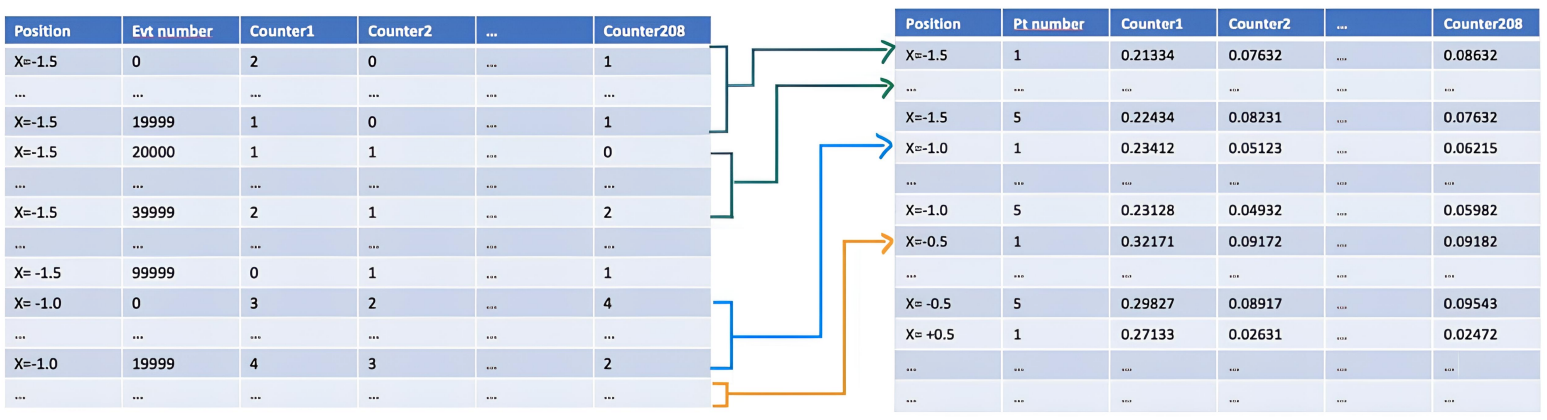
\includegraphics[width=\textwidth]{figures/tabular_dataset.png}
    \caption{Scheme of the last step in the creation of the tabular dataset used for estimating the PCA. An example regarding the x dataset is depicted. In the table on the left the dataset containing the raw events obtained from the simulation files are depicted. Notice that we have 100 thousand points for each nominal position and that the variables Counter1, Counter2, etc. indicate an integer, i.e. the number of clusters counted in that specific event by that specific counter. The tabular dataset on the right is obtained by integrating chunks of 20 thousand events at the same nominal position. Notice that in the dataset on the right we have 5 points per position, and that the features indicating the counters are float values that indicate the \textit{rate} of the counters, i.e. the mean number of clusters per event.}
    \label{fig:tabular_dataset}
\end{figure}

The very last step of this dataset creation procedure involves splitting each dataset in two, in order to create the final datasets: 
\begin{itemize}
    \item the train dataset: in the training dataset only the first 2 points per position are kept. We end up with a dataset containing 12 entries for $x$ and $y$, and 24 entries for $z$. For the sake of clarity, let us name these datasets respectively $\mathbf{X}_{train}$, $\mathbf{Y}_{train}$ and $\mathbf{Z}_{train}$.  This dataset is used to estimate the weights $\mathbf{w}_{(k)}$ as it will be described in the next section.
    \item the test dataset: in the test dataset the last 3 points per position are stored. These datasets comprehend 18 entries for $x$ and $y$, and 36 entries for $z$. For the sake of clarity, let us name these datasets respectively $\mathbf{X}_{test}$, $\mathbf{Y}_{test}$ and $\mathbf{Z}_{test}$. These points are used to estimate the scores $\mathbf{t}_{(i)}$ and asses their relationship with the beamline position. By fitting this yet-to-discover relationship we can also calculate the residuals in order to estimate the resolution of the estimators.
\end{itemize}


\section{Creating the estimators on MC}

We want to construct three different quantities $\hat{x}$, $\hat{y}$, $\hat{z}$ to estimate the beamline position components using $l$ scores $t_k$ derived with the PCA algorithm.
\begin{align}
\begin{split}
    \hat{x} &= \hat{x}(t^x_1, \dots, t^x_l) \\
    \hat{y} &= \hat{y}(t^y_1, \dots, t^y_l) \\\label{x_hat}
    \hat{z} &= \hat{z}(t^z_1, \dots, t^z_l) 
    \end{split}
\end{align} 

Each one of the scores $t_k$ is described by \eqref{score}, hence we need to properly define $\mathbf{x}_{(i)}$ and $\mathbf{w_{(k)}}$. The $\mathbf{x}_{(i)}$ vector is a 208-dimensional vector containing the mean cluster counts per events on each one of the $p$ implemented counters. The  $\mathbf{w_{(k)}}$ is the vector of weights for calculating the $k$-th component with the PCA algorithm and we will use the $\mathbf{X}_{train}$, $\mathbf{Y}_{train}$ and $\mathbf{Z}_{train}$ datasets to estimate them. As described in Section \ref{sec:PCA}, we calculate the covariance matrices of these datasets and we diagonalize them in order to get $k$ 208-dimensional weights vectors $\mathbf{w_{(k)}}$, that represent the new basis of the space computed by the PCA. 
Once the diagonalization is performed, the eigenvalues of the covariance matrices offer a first statistics to look at. In figure \ref{fig:scree_plot} we report a scree plot, i.e. a bar chart displaying the normalised eigenvalues, which represents the percentage of variance explained by that specific component. As one can see, more than 90\% of the variance is explained by the first PC, while the others give marginal contributions. This plot suggest that probably only the first PC is enough to characterise the luminous region position.
\begin{figure}
    \centering
    \begin{subfigure}{0.48\textwidth}
    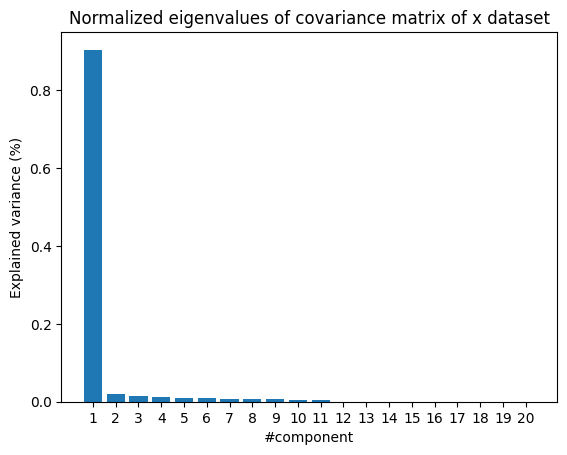
\includegraphics[width=\linewidth]{figures/x_eigenvalues.png}
    \caption{$x$ dataset}\label{fig:x_eigenvalues}
    \end{subfigure}
    \begin{subfigure}{0.48\textwidth}
    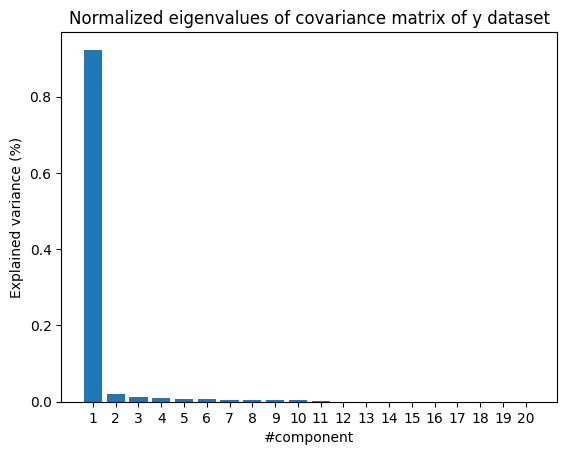
\includegraphics[width=\linewidth]{figures/y_eigenvalues.png}
    \caption{$y$ dataset}\label{fig:y_eigenvalues}
    \end{subfigure}
    \caption{Scree plot for the $x$ and $y$ dataset. For both datasets the first component explains more than 90\% of the variance, meaning that the first PC is probably enough to perform the beamline estimation.}
    \label{fig:scree_plot}
\end{figure}

 We can calculate the first PC scores $\mathbf{t^j}_{1(i)}$ as \eqref{first_score} using the test datasets $j$ for each $j=x,y,z$ coordinate, in order to check the relationships between $\mathbf{t^{j}}_{1(i)}$ and the luminous region positions. The scores are calculated using the rates $\mathbf{x^{j}_{(i)}}$ of the test datasets and the vectors $\mathbf{w^{j}}_{(1)}$ estimated from the train datasets. We use two different datasets in order to ensure that the vectors $\mathbf{w^{j}}_{(1)}$ do not provide a biased estimation towards the train datasets. Being the test datasets completely independent from the train datasets, we can asses the validity of this method. In fact,  the scores $\mathbf{t^{j}}_{1(i)}$ will be read online using the readout of the clustering $\mathbf{x_{(i)}}$ in real time and the vectors $\mathbf{w^{j}}_{(1)}$ will rely on the pre-calculated vectors in the MC. The relationship between the first PC calculated as \eqref{first_score} and the luminous region position can be assessed in the test datasets as depicted in the Figures \ref{fig:xfit_MC}, \ref{fig:yfit_MC}, \ref{fig:zfit_cubic_MC} for respectively the $x$, $y$ and $z$ components. As one can see, the relationship is linear for $x$ and $y$, while it is cubic for the $z$ displacements. In the Figures \ref{fig:xfit_MC}, \ref{fig:yfit_MC}, \ref{fig:zfit_cubic_MC} we also perform a best fit using the minimal $\chi^2$ method using a linear or cubic function to better validate this hypothesis. 
%\begin{figure}
%    \centering
%    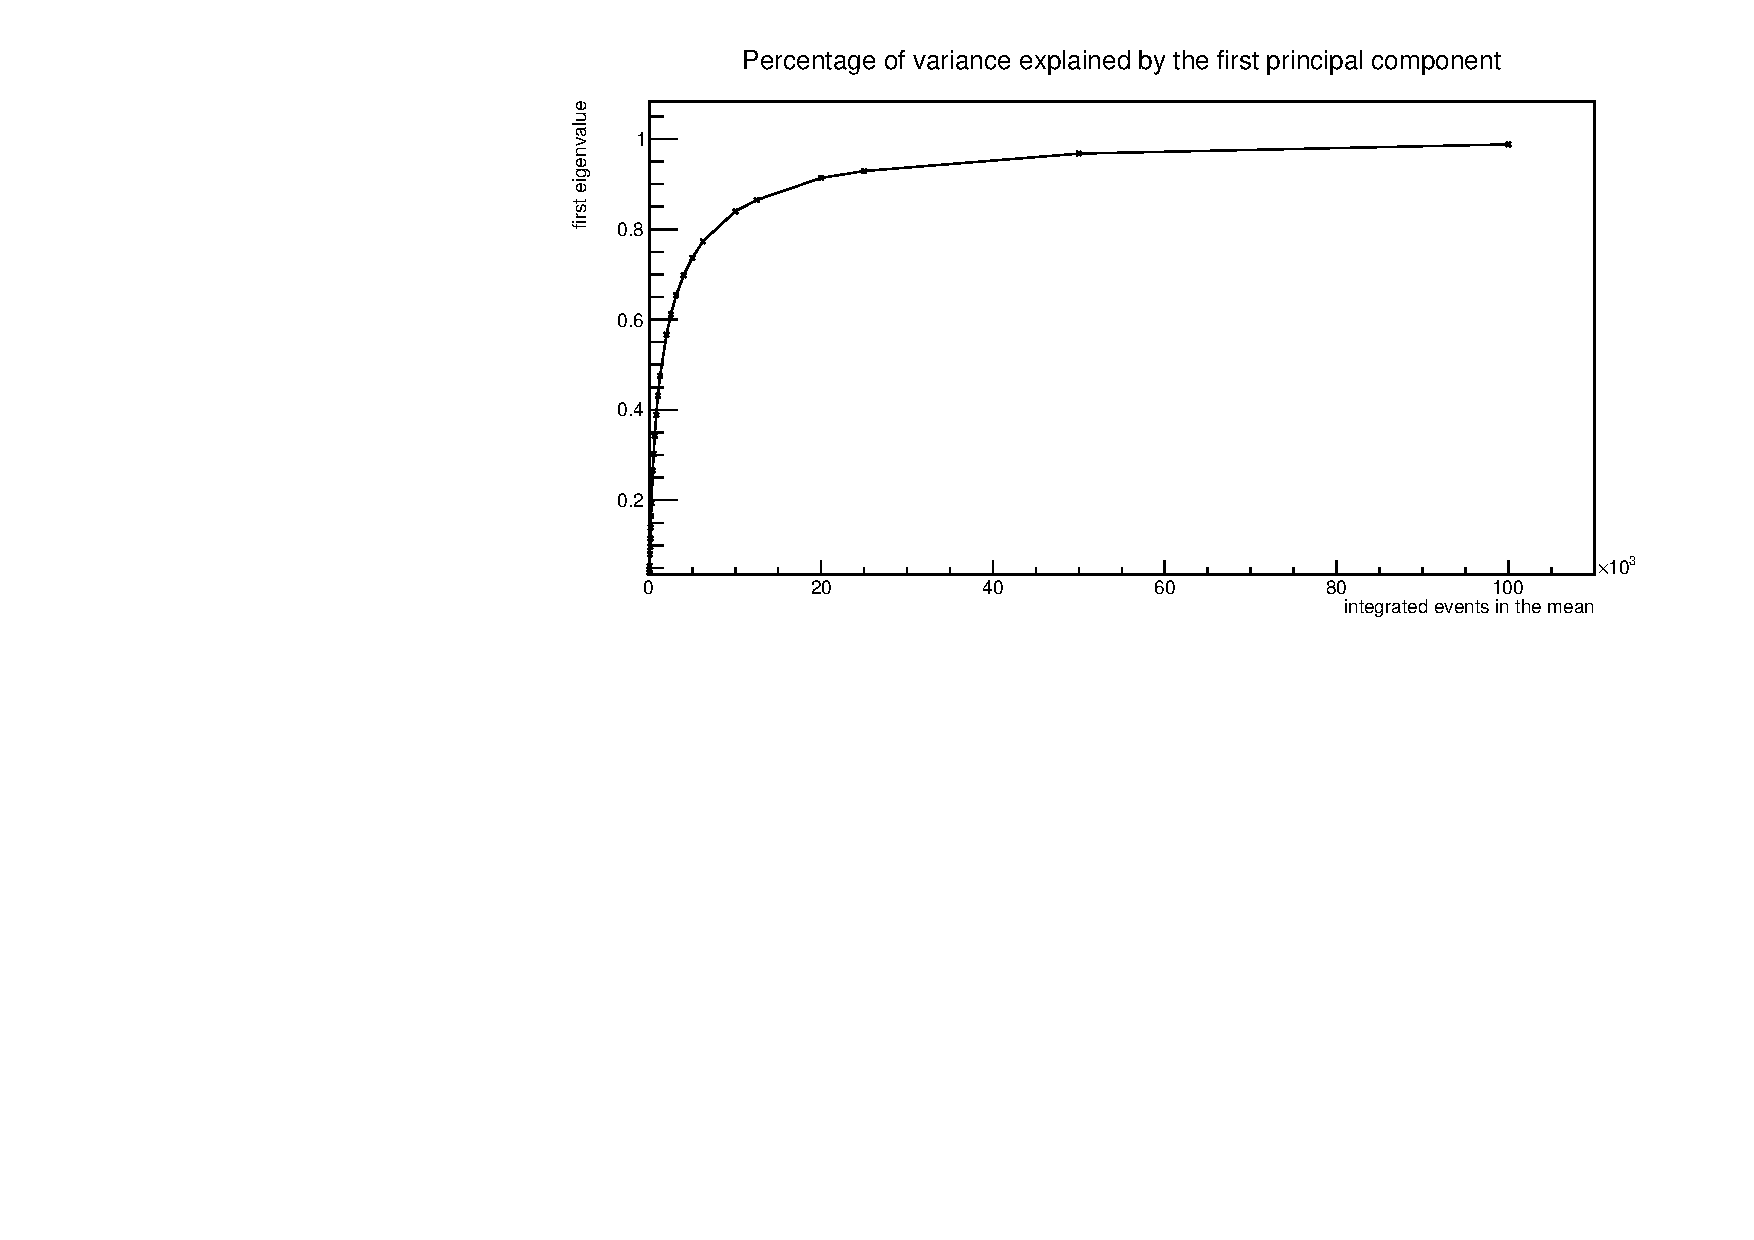
\includegraphics[width=\textwidth]{figures/explained_variance_new_y.pdf}
%    \caption{Percentage of explained variance varying the number of integrated events for computing the mean number of clusters per event.}
%    \label{fig:explained_variance}
%\end{figure}


\begin{figure}
    \centering
    \begin{subfigure}{0.48\textwidth}
    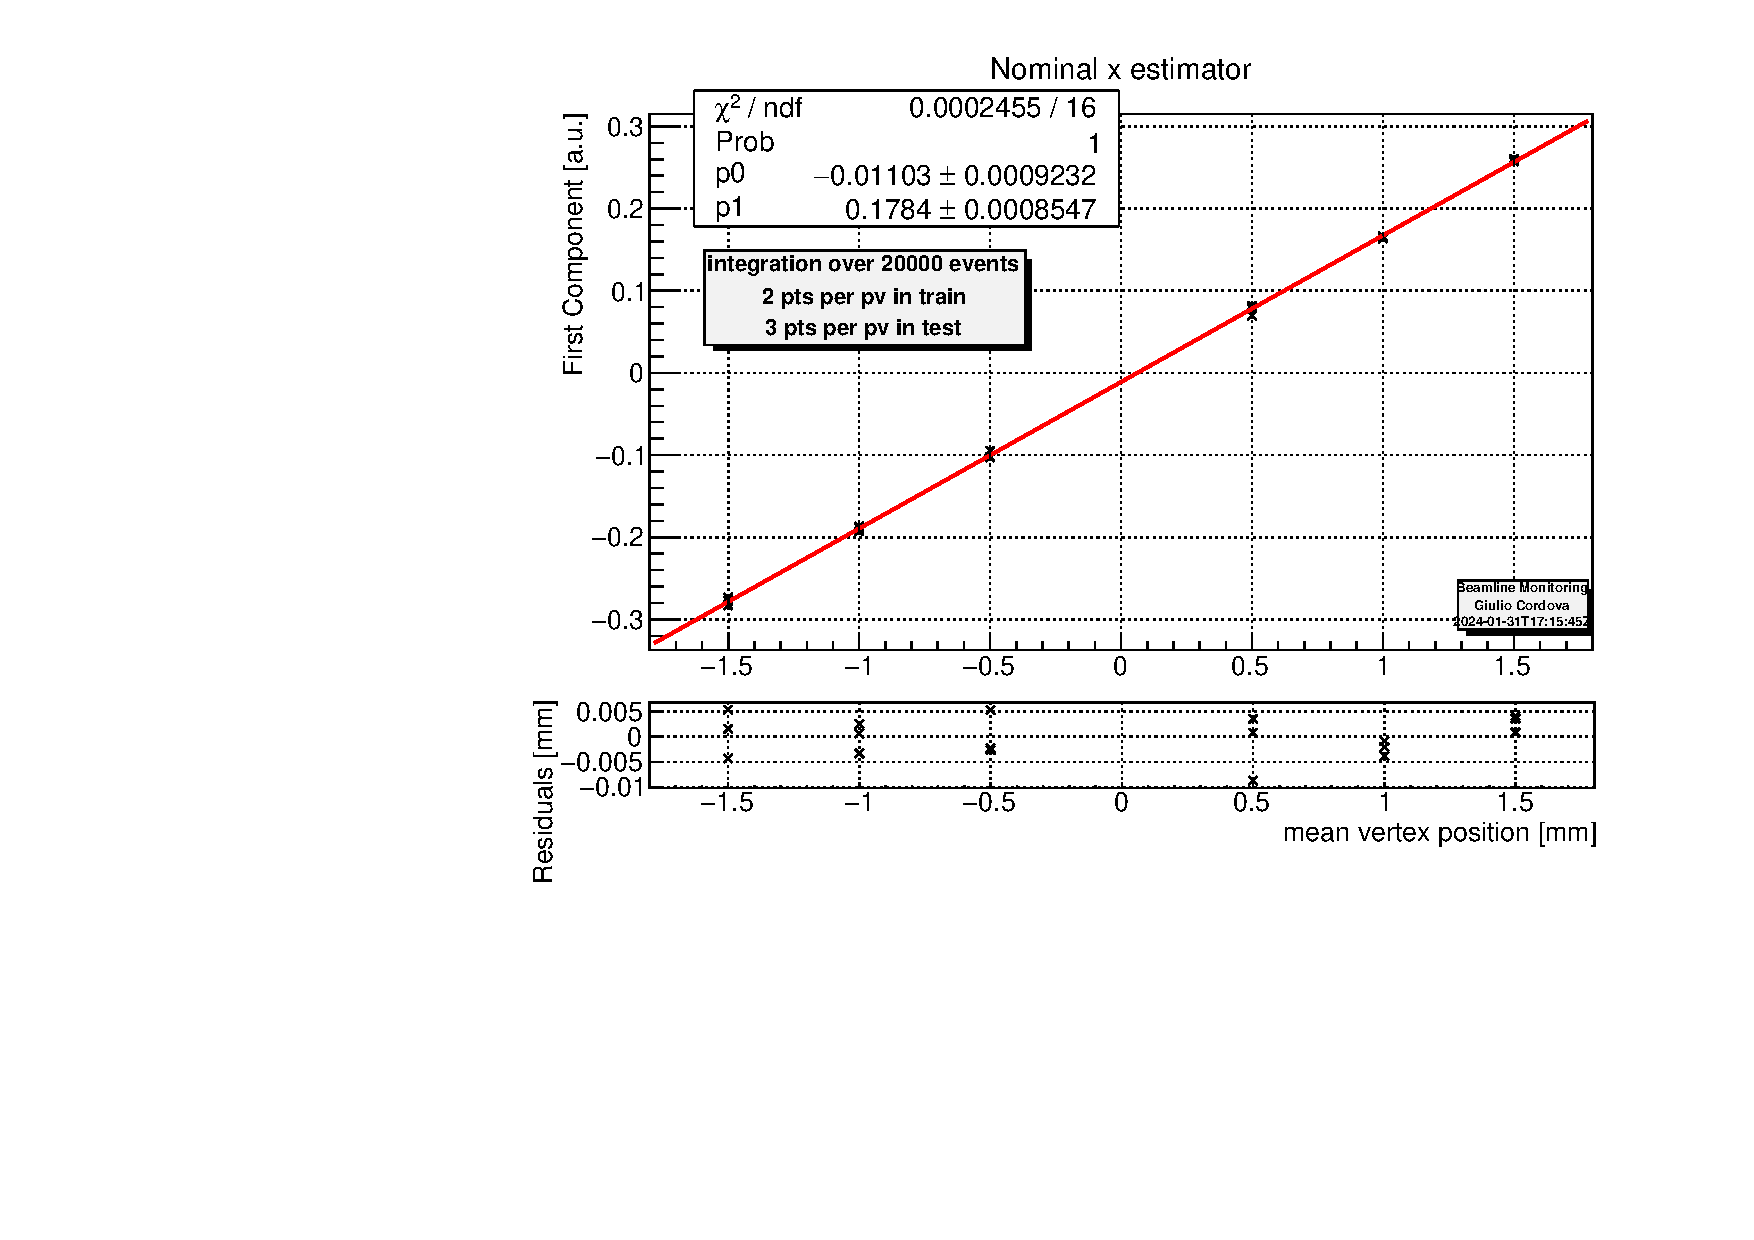
\includegraphics[width=\linewidth]{figures/x_fit_MC.pdf}
    \caption{Linear Fit}\label{fig:xfit_MC}
    \end{subfigure}
    \begin{subfigure}{0.48\textwidth}
    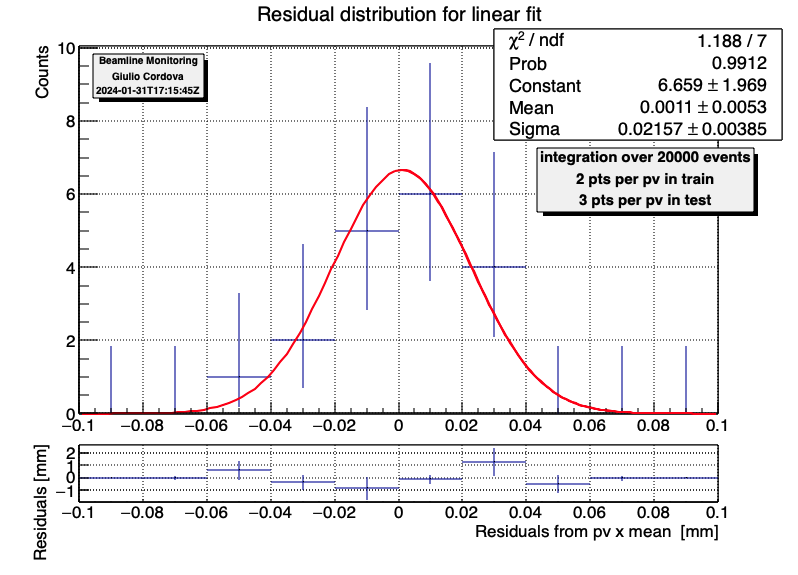
\includegraphics[width=\linewidth]{figures/x_res_MC.png}
    \caption{Residuals from the fit of the graph on the left. }\label{fig:xres_MC}
    \end{subfigure}
    \caption{Linearity of the first component calculated with the PCA with respect to luminous region position shifts in x component, alongside the residuals distribution fitted with a Gaussian distribution.}
    \label{fig:x_MC}
\end{figure}


\begin{figure}
    \centering
    \begin{subfigure}{0.48\textwidth}
    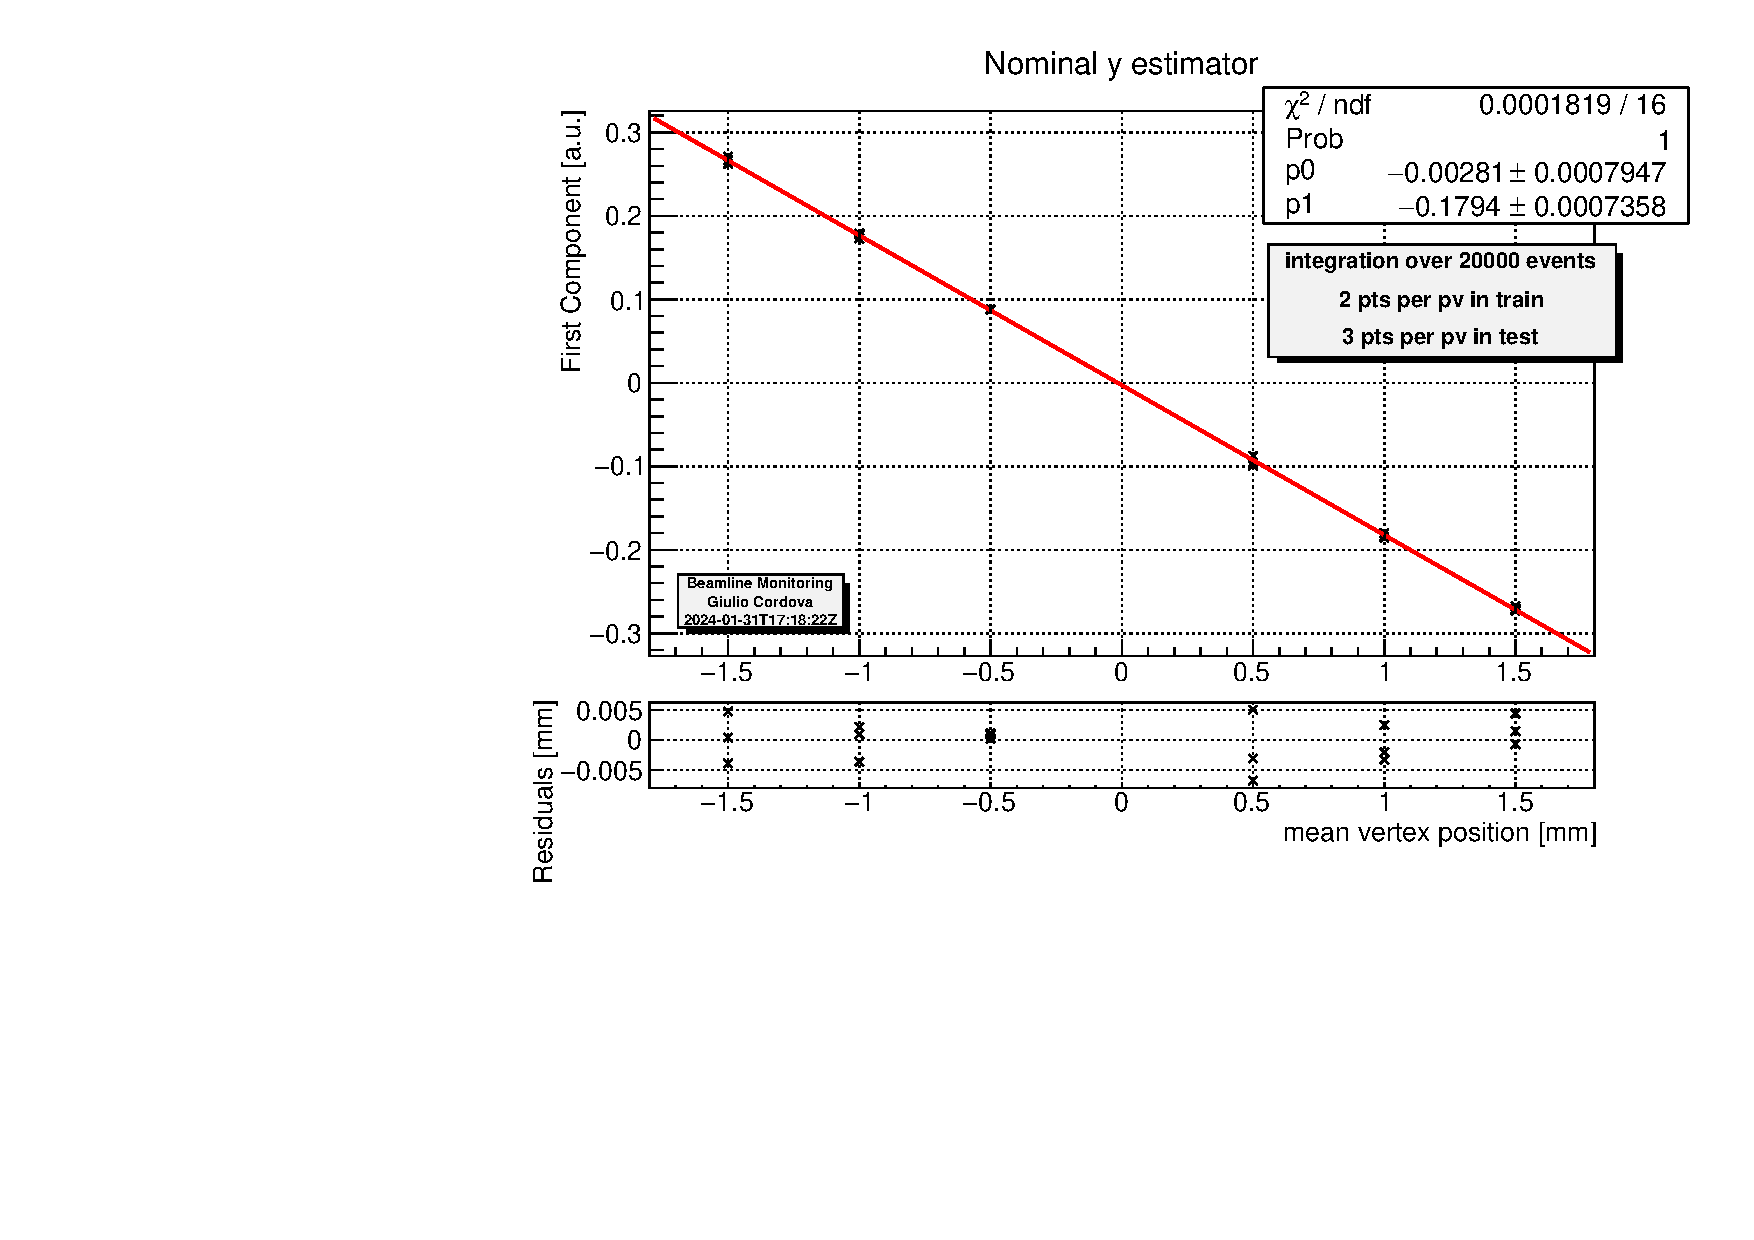
\includegraphics[width=\linewidth]{figures/y_fit_MC.pdf}
    \caption{Linear Fit}\label{fig:yfit_MC}
    \end{subfigure}
    \begin{subfigure}{0.48\textwidth}
    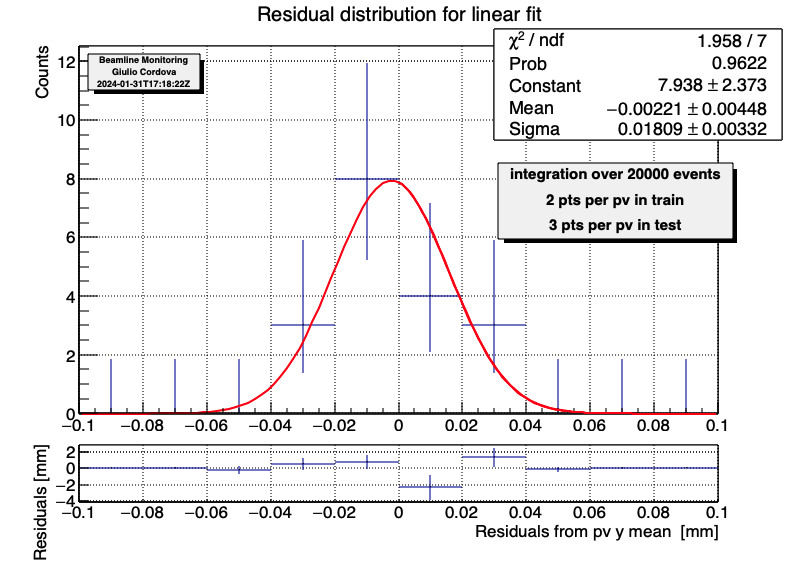
\includegraphics[width=\linewidth]{figures/y_res_MC.png}
    \caption{Residuals from the fit of the graph on the left. }\label{fig:yres_MC}
    \end{subfigure}
    \caption{Linearity of the first component calculated with the PCA with respect to luminous region position shifts in y component, alongside the residuals distribution fitted with a Gaussian distribution.}
    \label{fig:y_MC}
\end{figure}


\begin{figure}
    \centering
    \begin{subfigure}{0.48\textwidth}
    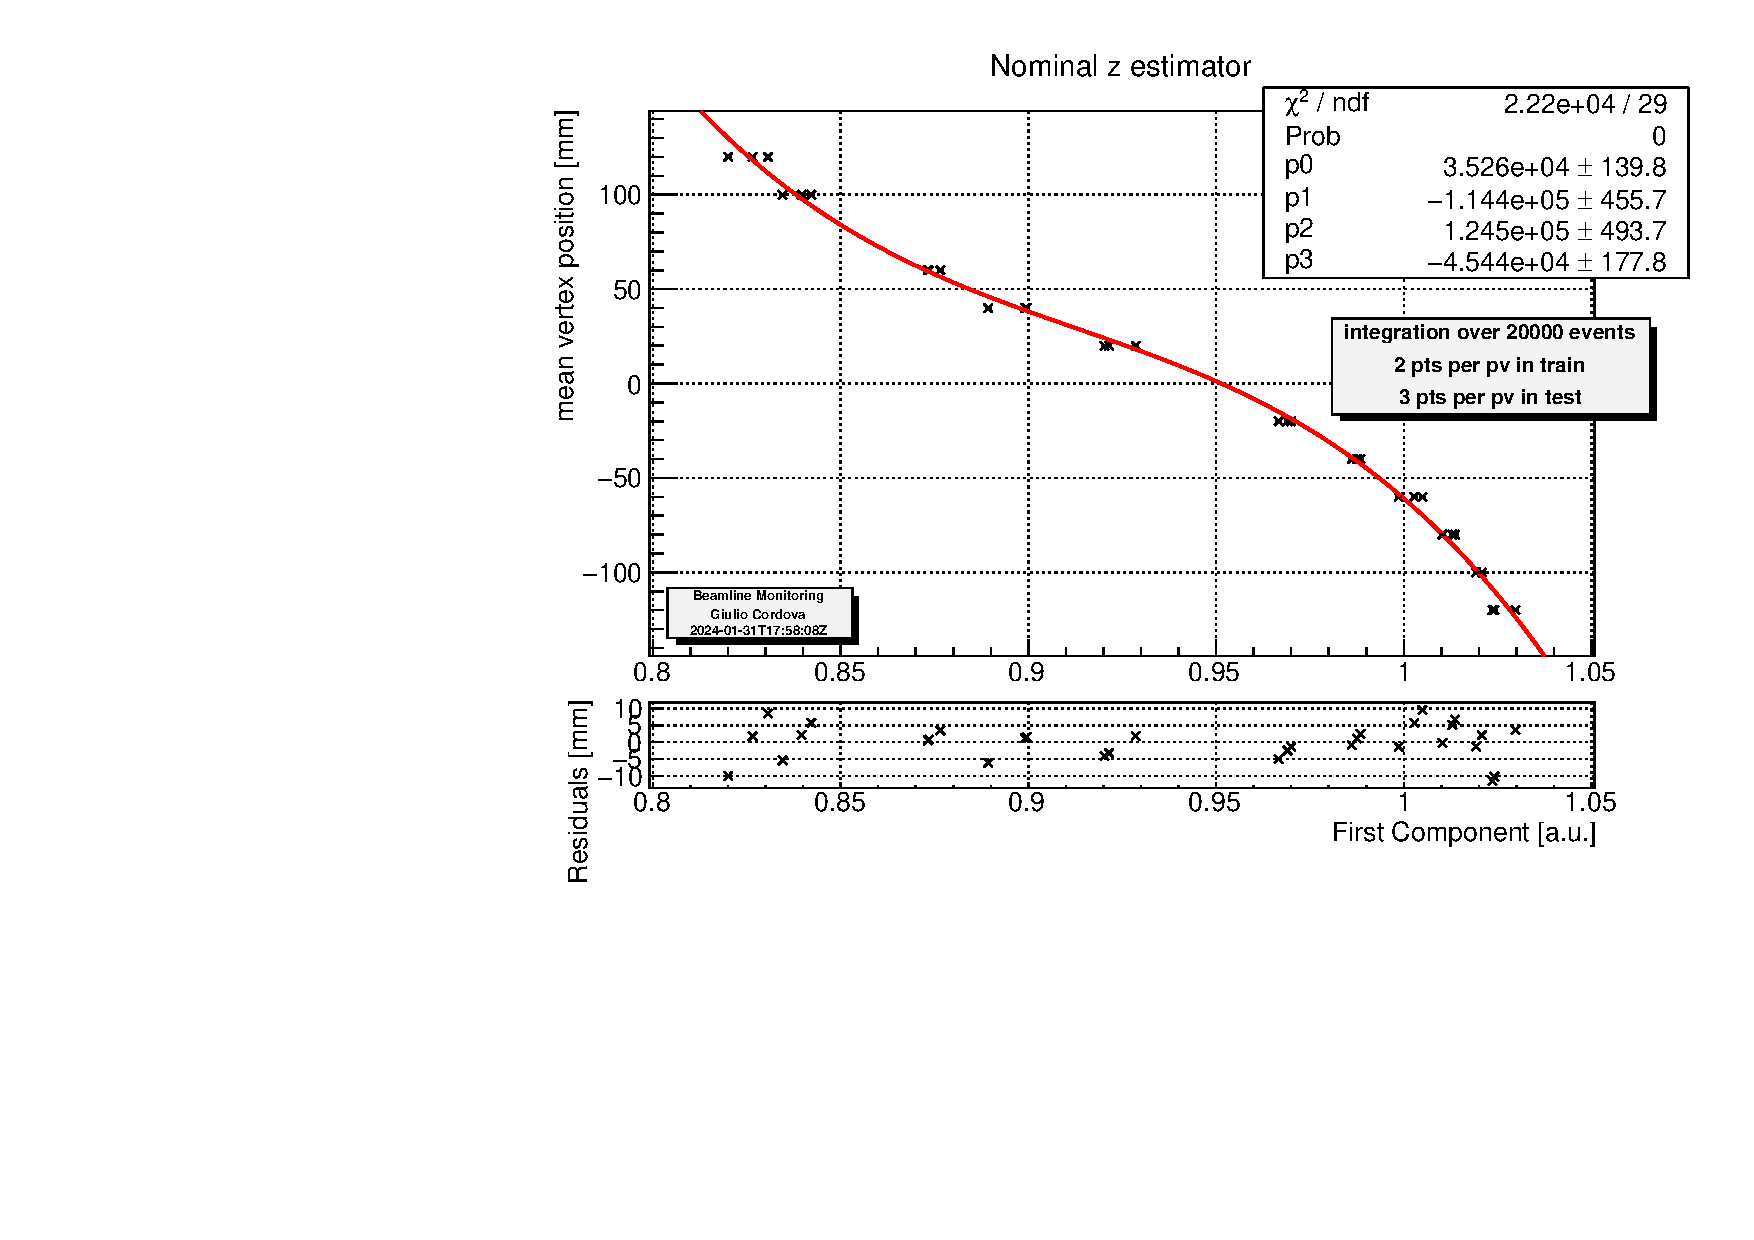
\includegraphics[width=\linewidth]{figures/z_cubic_fit.pdf}
    \caption{Cubic Fit}\label{fig:zfit_cubic_MC}
    \end{subfigure}
    \begin{subfigure}{0.48\textwidth}
    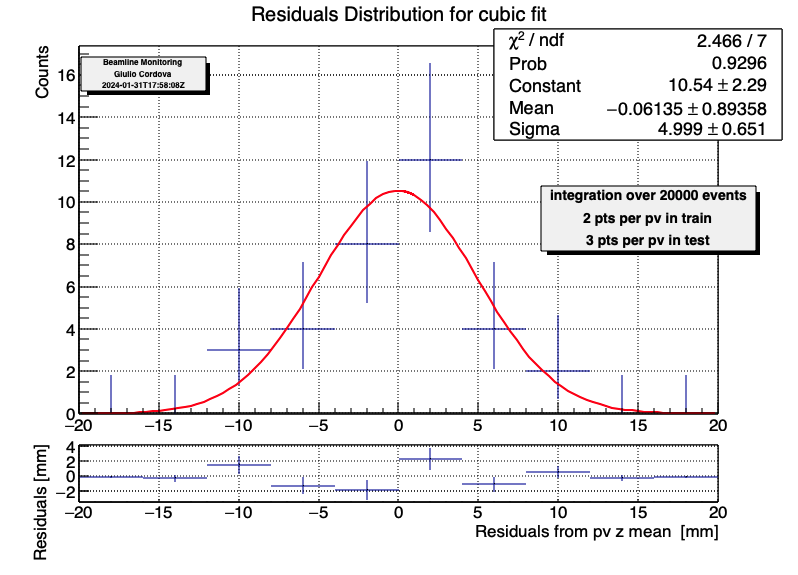
\includegraphics[width=\linewidth]{figures/z_cubic_res.png}
    \caption{Residuals from the fit of the graph on the left. }\label{fig:zres_cubic_MC}
    \end{subfigure}
    \caption{Cubic relationship between the first component calculated with the PCA and luminous region position shifts in z component, alongside the residuals distribution fitted with a Gaussian distribution.}
    \label{fig:z_cubic_MC}
\end{figure}

We can therefore rewrite \eqref{x_hat} as a simple quantity depending only on the first PC $\mathbf{t^j_1}$:
\begin{align}
\begin{split}
    \hat{x} &= \hat{x}(t^x_1) = a_x t^x_1 + b_x \\
    \hat{y} &= \hat{y}(t^y_1) = a_y t^y_1 + b_y \\\label{x_hat_true}
    \hat{z} &= \hat{z}(t^z_1) = a_z (t^z_1)^3 + b_z (t^z_1)^2 + c_z  t^z_1 + d,
    \end{split}
\end{align} 
with the various coefficients to be estimated directly from the fit performed. 

In the Figures \ref{fig:xres_MC}, \ref{fig:yres_MC}, \ref{fig:zres_cubic_MC} we report the histogram of the residuals $\mathbf{r}=(r_x, r_y, r_z)$ computed as 
 \begin{equation}
     \mathbf{r}=\hat{\mathbf{x}} - \mathbf{x_{true}} \qquad \text{with } \hat{\mathbf{x}} = (\hat{x}, \hat{y}, \hat{z}) \quad \text{ and } \quad \mathbf{x_{true}}=(x_{true}, y_{true}, z_{true}).
 \end{equation}

 Each one of the histograms is fitted with a Gaussian distribution, in order to provide also a resolution of the estimation. The errorbars of this histograms are asymmetrical confidence intervals at $67$\% of the Poisson counts in the bin.
 As one can see, the resolution is quoted to be around \SI{20}{\micro\meter} for $x$ and $y$ component, while we quote a resolution of \SI{5}{\milli\meter} for the $z$ component. We expect to have a worse resolution in $z$ compared to the ones in $x$ and $y$ because the luminous region is more spread in this direction, as explained in the description of the dataset in Section \ref{sec:MC}.
 \paragraph{On the estimated resolution}
 The resolution that we quote here depends on the two factors that we need to estimate $\mathbf{t^{j}}_{1}$, i.e. the vector of weights $\mathbf{w^j}_{(1)}$ and the mean number of clusters per event in each counter $\mathbf{x^{j}}$. As already stated, the counters are Poisson counts with mean depending on the position of the counter and the luminous region position. In first approximation we can treat the counters as independent variables, hence each counter $c_k$ follows a Poisson distribution with mean $\lambda_k$
 \begin{equation}
     f(c_k) = \frac{e^{-\lambda_k} \mu^{c_k}}{c_k!}
 \end{equation}

The MLE for the parameter $\lambda$ of a Poisson distribution is simply given by the sample mean $\bar{c}=\frac{\sum_i c^i}{N}=x$. 
 Since the Poisson is additive, the distribution of the sum of N independent counts of the same counters is still a Poisson distribution with mean $N\lambda_k$
 \begin{equation}
     f\bigl(\sum_i c^i_k\bigr) = \frac{e^{-N\lambda_k} \mu^{\sum_i c^i_k}}{(\sum_i c^i_k)!}
 \end{equation}
Therefore, the sample mean follows still a Poisson distribution with parameter $N\lambda_k$. The variance associated to the sample mean and therefore to mean number of counts per event in each counter $k$:
\begin{equation}
    \text{Var}(x_k) =\text{Var}\biggl(\frac{\sum_i c^i_k}{N}\biggr) = \frac{\lambda_k}{N}
\end{equation}

The contribution to the uncertainty given by the weights $\mathbf{w^j}_{(1)}$ is much more complicated, because its estimation depends on the diagonalization process. One way to estimate the variance on the $\mathbf{w^j}_{(1)}$ would be a  bootstrap\cite{10.1214/aos/1176344552} over multiple copies of PCAs, performed generating the points $\mathbf{x^{j}}$ from a 208-dimensional Gaussian distribution defined in \eqref{mvgaussian} using as parameters the data-inferred means $\mathbf{\lambda}$ and covariance matrix $\mathbf{\Sigma}$.  For the purpose of this thesis, this exercise was not performed, but this is of utterly importance for a more refined estimator.

By considering the Poisson uncertainty, only the number of integrated events $N$ influences the statistical error. In the case of Monte Carlo simulation presented in this thesis, we integrated over $N=2\cdot10^{4}$ events at $\mu=5.5$, that in Physics conditions (trigger rate $f=\SI{23}{\mega\hertz}$) corresponds to performing a measurement every $N/f=\SI{870}{\micro\second}$, corresponding to a frequency $\SI{1.5}{\kilo\hertz}$. As it will be shown in the following section of data testing, the resolution will increase due to the augmented statistics used for computing the mean cluster counts per event.

\paragraph{On the dependency on $\mu$}\label{sec:mu_dependency}
All the counters are linear dependent to the mean interaction per event $\mu$ as presented in chapter \ref{chap:luminosity}. If we have a change in $\mu$, the counters values will change accordingly. Since we use the counters to estimate the luminous region position, the estimate performed will be biased by the $\mu$ quantity. In order to check how the change in $\mu$ affects our luminous region estimate, we make use of the simulations 
of point (iv) of section \ref{sec:MC}. These simulations comprehend four different scans in a $\mu$ range that varies from $\nu=7.6$ to $\nu=35.8$\footnote{The linear relationship between the mean number of interactions per event $\mu$ and the mean number of PVs $\nu$ is given by the factor $\tfrac{\mu}{\nu}=\frac{5.5}{7.6}\approx 0.72$}, all at the nominal beam position at $0$ in the three Cartesian components. 
The relationship between the luminous region estimate and $\mu$ can be assessed by calculating the luminous region position using $\ref{x_hat_true}$. Since the position is set at $(0,0,0)$~mm for each event in this simulations, we should always estimate $(0,0,0)$~mm. However, as one can notice from the Figures \ref{fig:x_to_lumi}, \ref{fig:y_to_lumi} and \ref{fig:z_to_lumi}, the estimation is linearly biased by the pile-up $\nu$, as expected. 
\begin{figure}
    \centering
    \begin{subfigure}{0.31\textwidth}
    \centering
    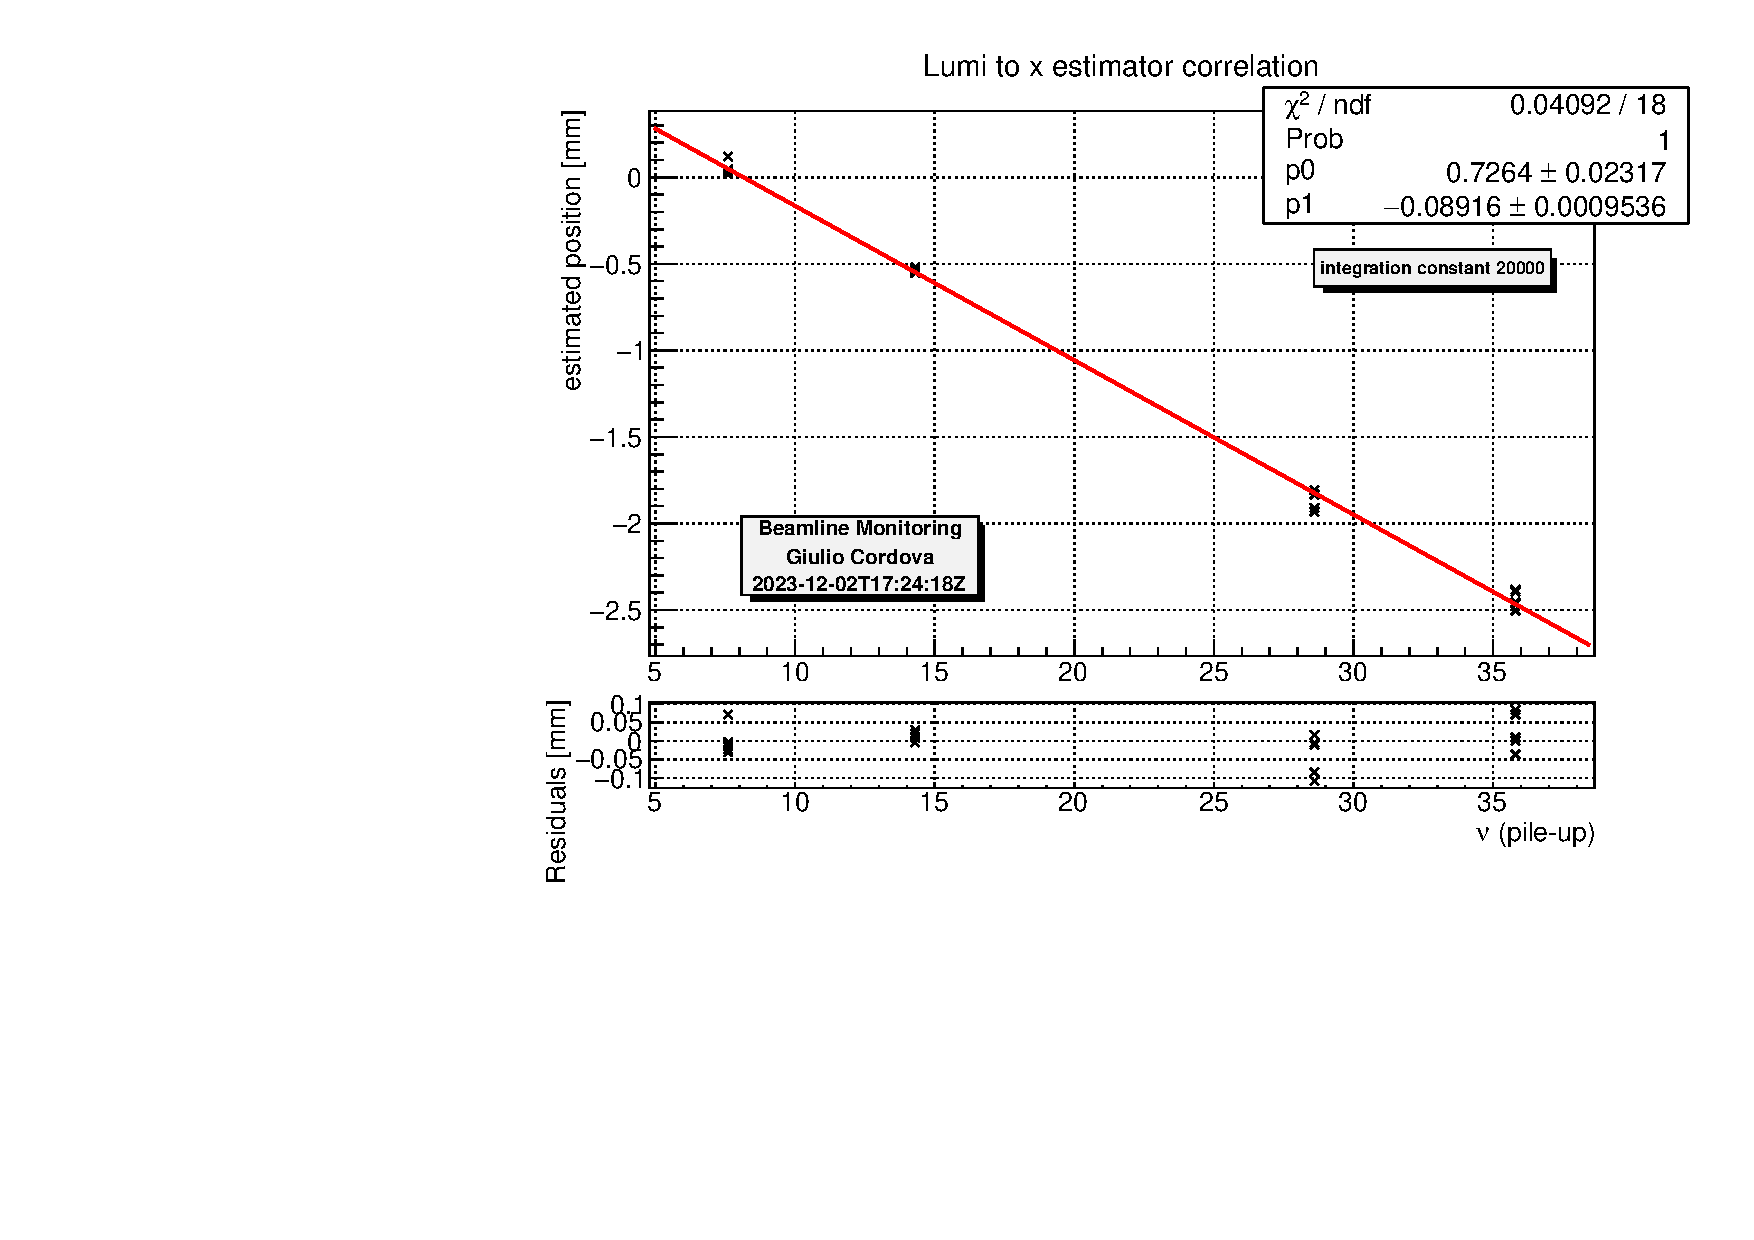
\includegraphics[width=\linewidth]{figures/x_to_lumi_fit_20000.pdf}
    \caption{$x$ component}
    \label{fig:x_to_lumi}
    \end{subfigure}\hfill
    \begin{subfigure}{0.31\textwidth}
    \centering
    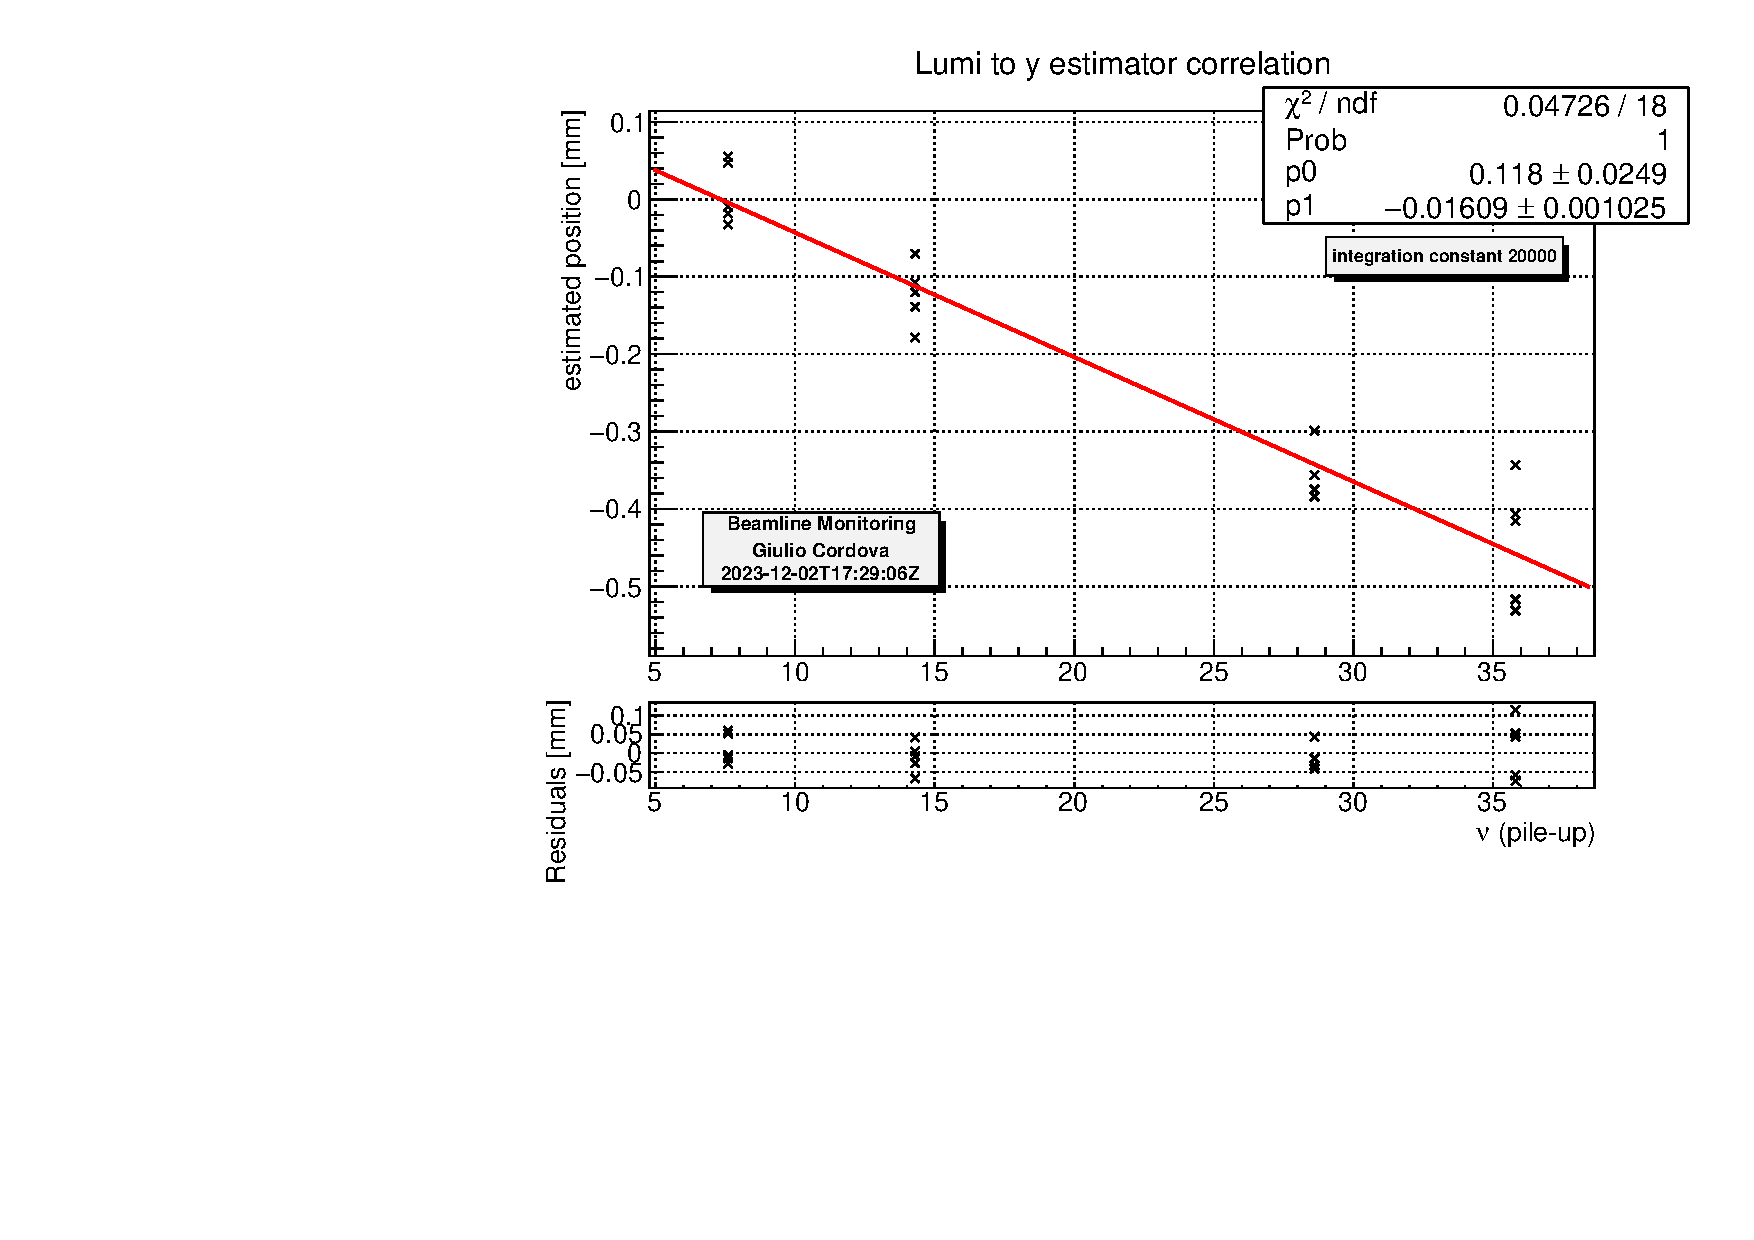
\includegraphics[width=\linewidth]{figures/y_to_lumi_fit_20000.pdf}
    \caption{$y$ component}
    \label{fig:y_to_lumi}
    \end{subfigure}\hfill
    \begin{subfigure}{0.31\textwidth}
    \centering
    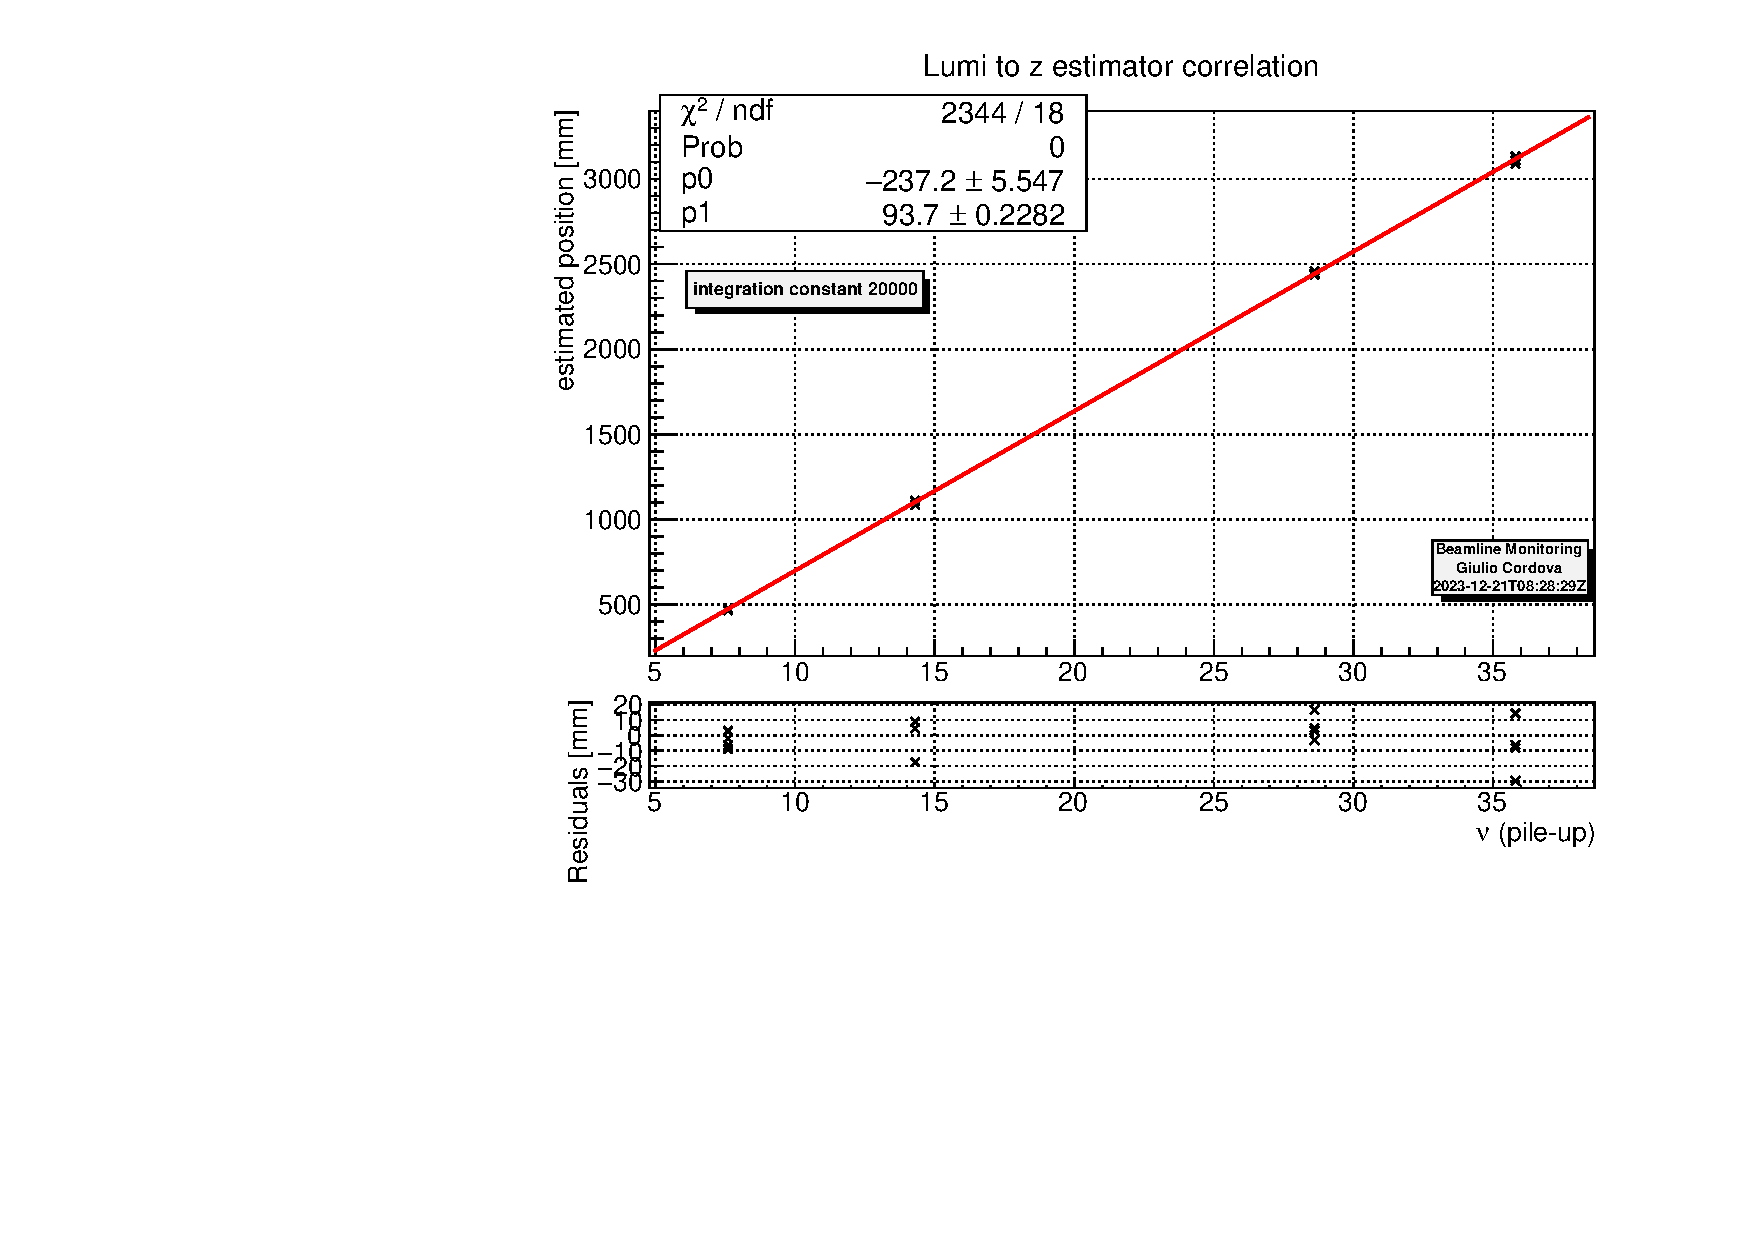
\includegraphics[width=\linewidth]{figures/z_to_lumi_fit_20000_numpix.pdf}
    \caption{$z$ component}
    \label{fig:z_to_lumi}
    \end{subfigure}
    \caption{Linear relationship between each component of the estimated position and pile-up $\nu$}
\end{figure}
The fact that the relationship is linear, offers us a straightforward way to correct for this bias. If we redefine the luminous region estimators as
\begin{equation}
\begin{split}
    \hat{x}_{corrected} &=\frac{\hat{x}(t^x_1)}{\mu}= a_x ' \frac{t^x_1}{\mu} + b_x '\\%\qquad
    \hat{y}_{corrected} &=\frac{\hat{y}(t^y_1)}{\mu}= a_y ' \frac{t^y_1}{\mu} + b_y ' \\%\qquad
    \hat{z}_{corrected} &=\frac{\hat{z}(t^z_1)}{\mu}=  a_z '\biggl(\frac{t^z_1}{\mu}\biggr)^3 + b_z '\biggl(\frac{t^z_1}{\mu}\biggr)^2 + c_z ' \frac{t^z_1}{\mu} + d ' \label{x_hat_corrected}
    \end{split}
    \end{equation}
we end up with unbiased estimators of the luminous region.



\section{Calibration and testing on collision data}
%\textit{Results obtained during VdM}
Once we have a suitable configuration in MC, we can perform a calibration and some tests on real collision data. The calibration is performed directly on the data because the available simulations used to estimate referred to 2022 conditions. Although these conditions do not differ much from the ones in 2024, the VELO was entirely uninstalled and reinstalled during the 2023 Year End Technical Shutdown (YETS), and completely reconfigured. These reconfiguration may introduce changes in efficiencies of the single sensors, therefore we decided to perform the calibration directly on the data. A suitable environment for the calibration is a sequence known as the Length Scale Calibration (LSC), typically part of the VdM scan fill for the determination of the beam sizes and their separation \cite{Balagura_2021}, which are parameters needed to compute the luminosity. During this sequence, the two beams are moved head-on from an initial position along the x-axis $x = -a$ to an end position $x = +a$, with respect to the nominal interaction position set at $x=0$. An analogue scan is repeated along the y-axis from $y=-a$ to $y=+a$. 
Given the beam movements in LSC, the estimators for the $x$ and $y$ component of the luminous region should be able to track it, following these scans.

\begin{figure}
    \centering
    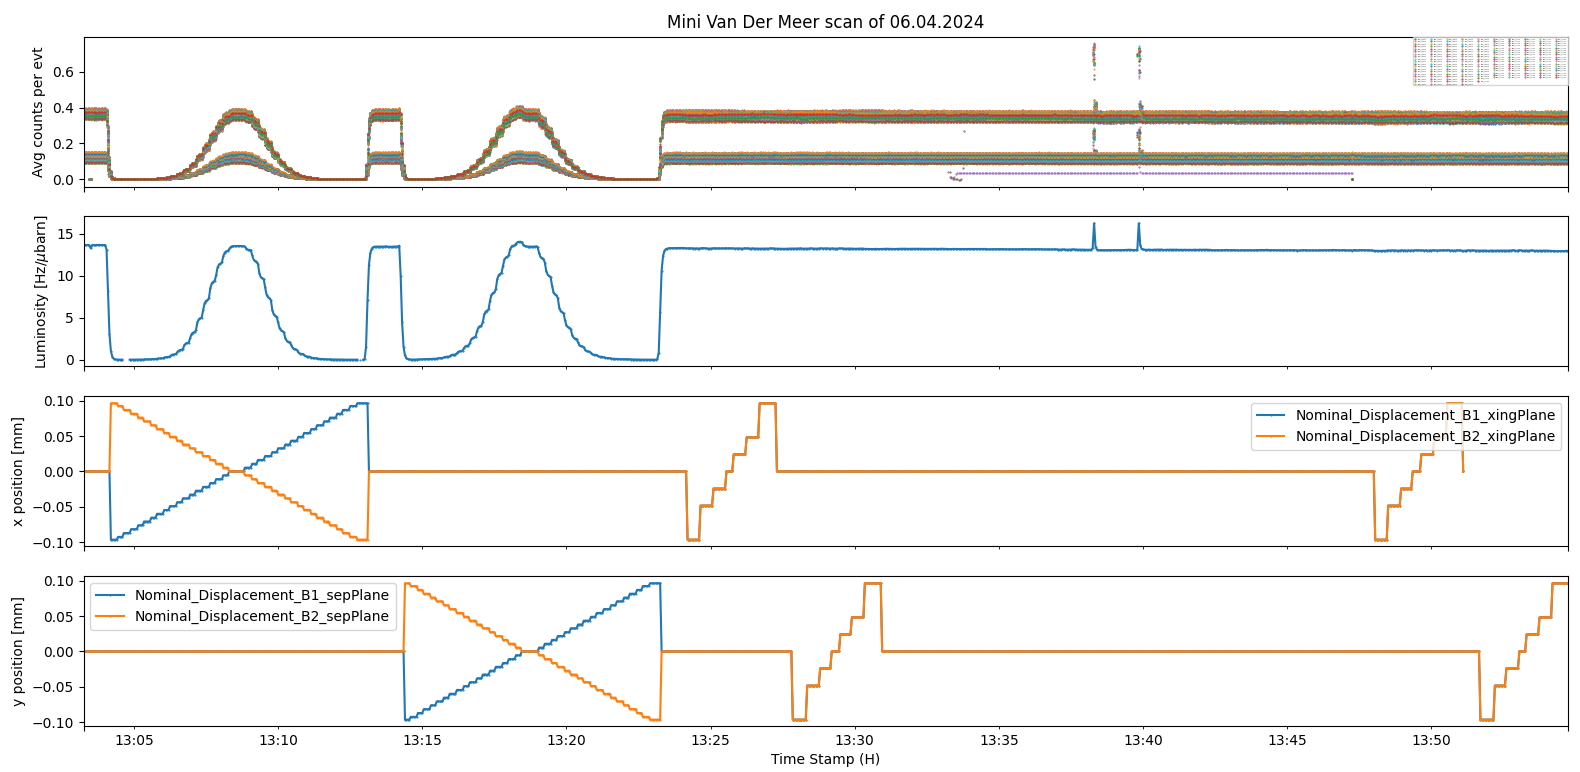
\includegraphics[width=\textwidth]{figures/lumi_with_counters.png}
    \caption{Overview of the mini Van Der Meer scan of April 6th, 2024. In the first panel we report the output of the counters as read in WinCC every three seconds, in the second panel the luminosity estimation performed using the trimmed mean as described in Chapter \ref{chap:luminosity}, while in the third and fourth panel the position of the two colliding beams in the $x$ and $y$ plane respectively.}
    \label{fig:mini-vdm}
\end{figure}

The LSC used for the presented calibration is the one performed on April, 6th 2024, with Fill ID 9475. In this Fill, we have 8 collisions bunches at an average $\mu=8.5$. In this scan, there were 4 scans performed. First a scan in X is performed, followed almost immediately by a scan in Y. After a rest time of approximately 20 minutes where there were no beamline movements, an additional sequence of scan in X and Y is performed, with the same parameters. The sequence is clearly visible in the plot of Figure \ref{fig:mini-vdm}, where in the third and fourth panel we can appreciate the movements of both beams (orange and blue) in the $x$ and $y$ plane, respectively. After the Symmetric VdM scan in both $x$ and $y$, a first LSC in $x$ is performed at approximately 13:25, followed by an analogue scan in the $y$ plane. A second LSC sequence is then performed around 13:47. In the first panel of Figure \ref{fig:mini-vdm} we also report the output of the rate of 208 counters as it is read by the TELL40s every 3 seconds, while on the second panel we report the luminosity estimate computed a-posteriori as the trimmed mean of the 208 luminosity estimate performed by each counter. The first VdM sequence is also used to calibrate the counters as described in section \ref{sec:calibration_vdm} for this luminosity estimation. 

Each readout $i$ of the cluster compose the 208-dimensional array $\mathbf{x}_i$ that is multiplied by the corresponding weight vector $\mathbf{w^j}_{(1)}$ computed in MC, for the estimation of the first PC score $\mathbf{t^j}_{(1)}$ that will be used to perform the estimation of the luminous region position in each component $j=x,y$. 

As observed in Section \ref{sec:mu_dependency}, the unbiased scores can be obtained by dividing the calculated $\mathbf{t^j}_{(1)}$ by the value of instantaneous $\mu$ of \eqref{inst_mu} calculated starting from the luminosity estimate provided by the trimmed mean.
The final estimator needs to be calibrated by computing the correct coefficients of equations \ref{x_hat_corrected}. This can be done by computing a linear fit between the true position of the beamline and the corrected scores $\mathbf{t^j}'_{(1)}=\mathbf{t^j}_{(1)}/\mu$. As true position, we use the position of primary vertices reconstructed by VELO monitoring tasks, providing an indication of the average position of the luminous region relative to the VELO. These monitoring tasks do not operate in real-time, but they provide about one position estimate per second a-posteriori, offering a solid basis for comparison with my estimators. After the matching between the Timestamp of these series is performed, we perform a comparison of the two data points during the first ramp in both $x$ and $y$. A result of this comparison s shown in the scatter plots of Figure \ref{fig:xfit_data} for the $x$ variable and Figure \ref{fig:yfit_data} for $y$ variable. The relationship is still linear, and the coefficients for the $\hat{x}_{corrected}$ and $\hat{y}_{corrected}$ can be estimated directly from this fit.

\begin{figure}
    \centering
    \begin{subfigure}{0.48\textwidth}
    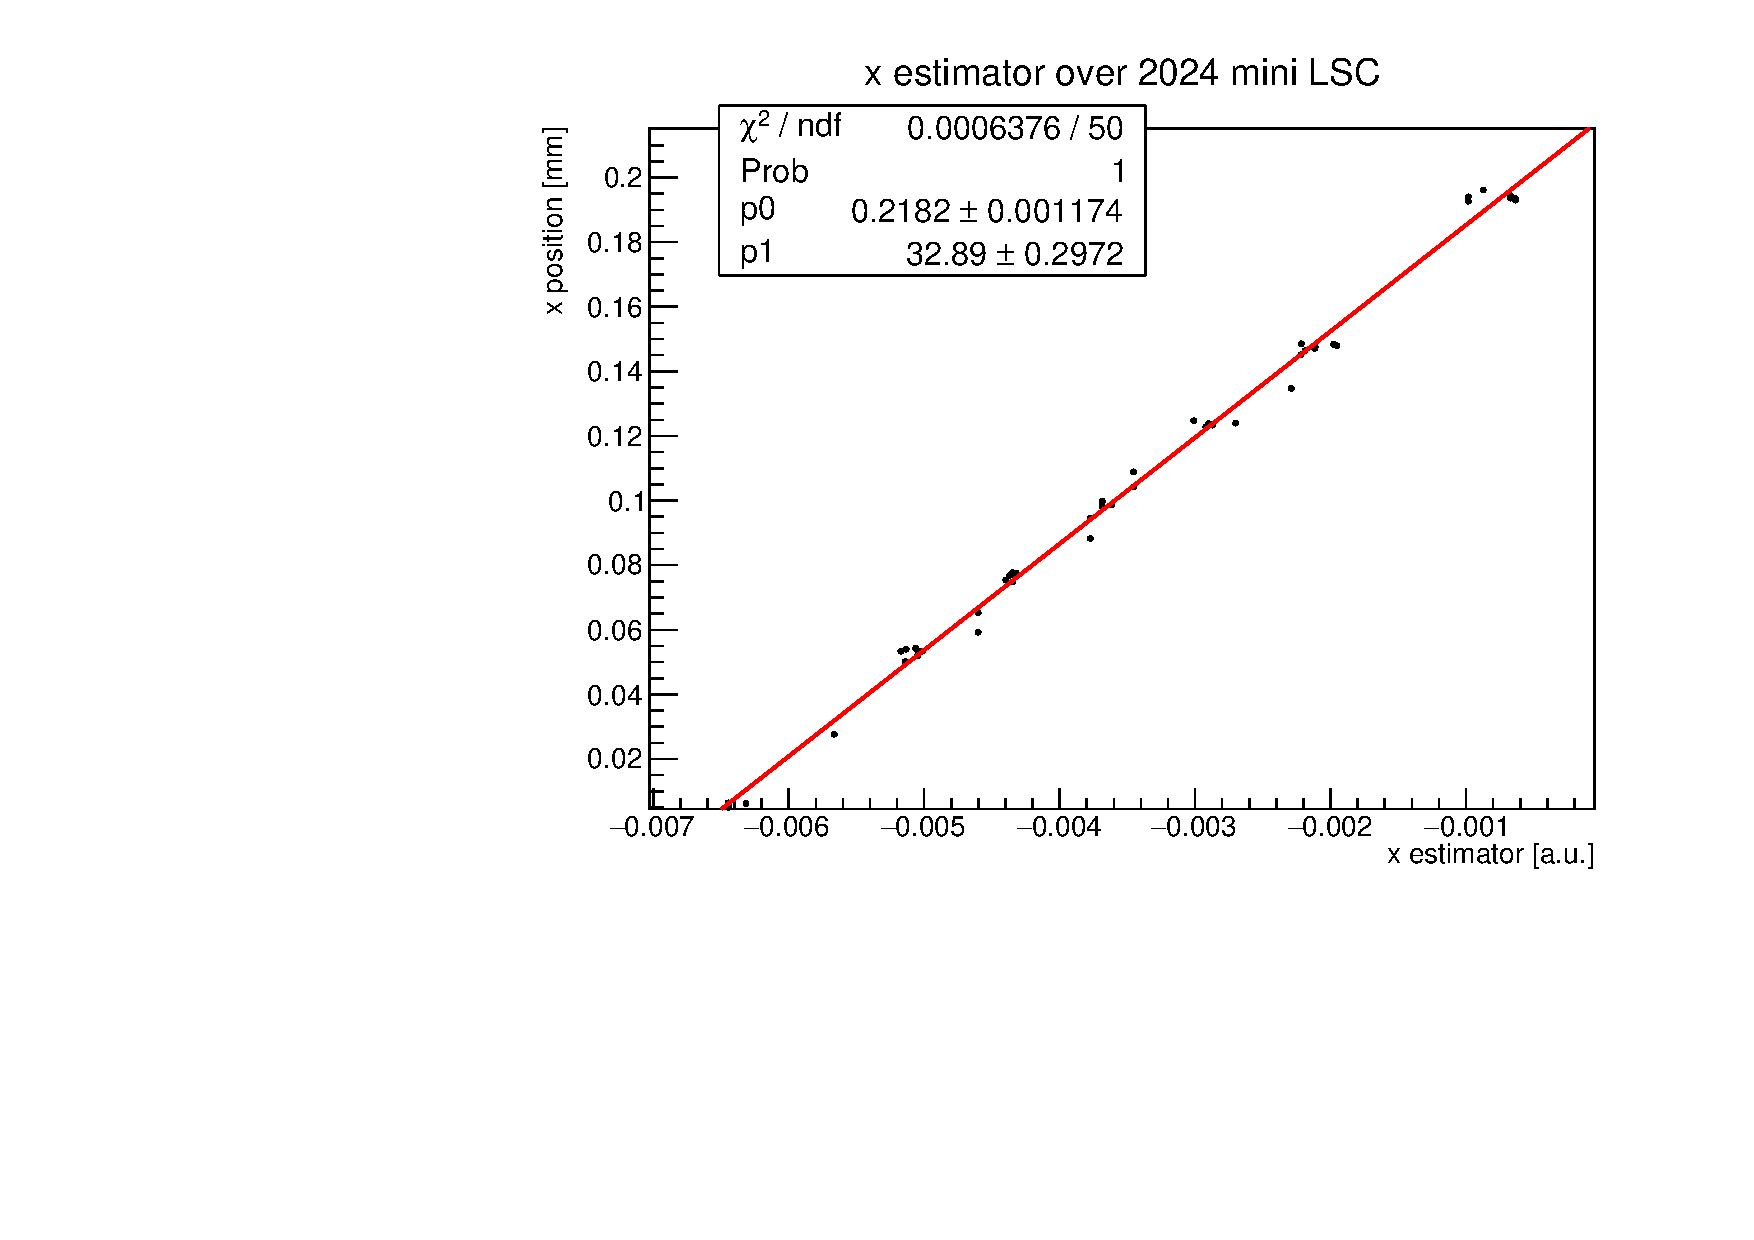
\includegraphics[width=\linewidth]{figures/x_res_new.pdf}
    \caption{Linear Fit}\label{fig:xfit_data}
    \end{subfigure}
    \begin{subfigure}{0.48\textwidth}
    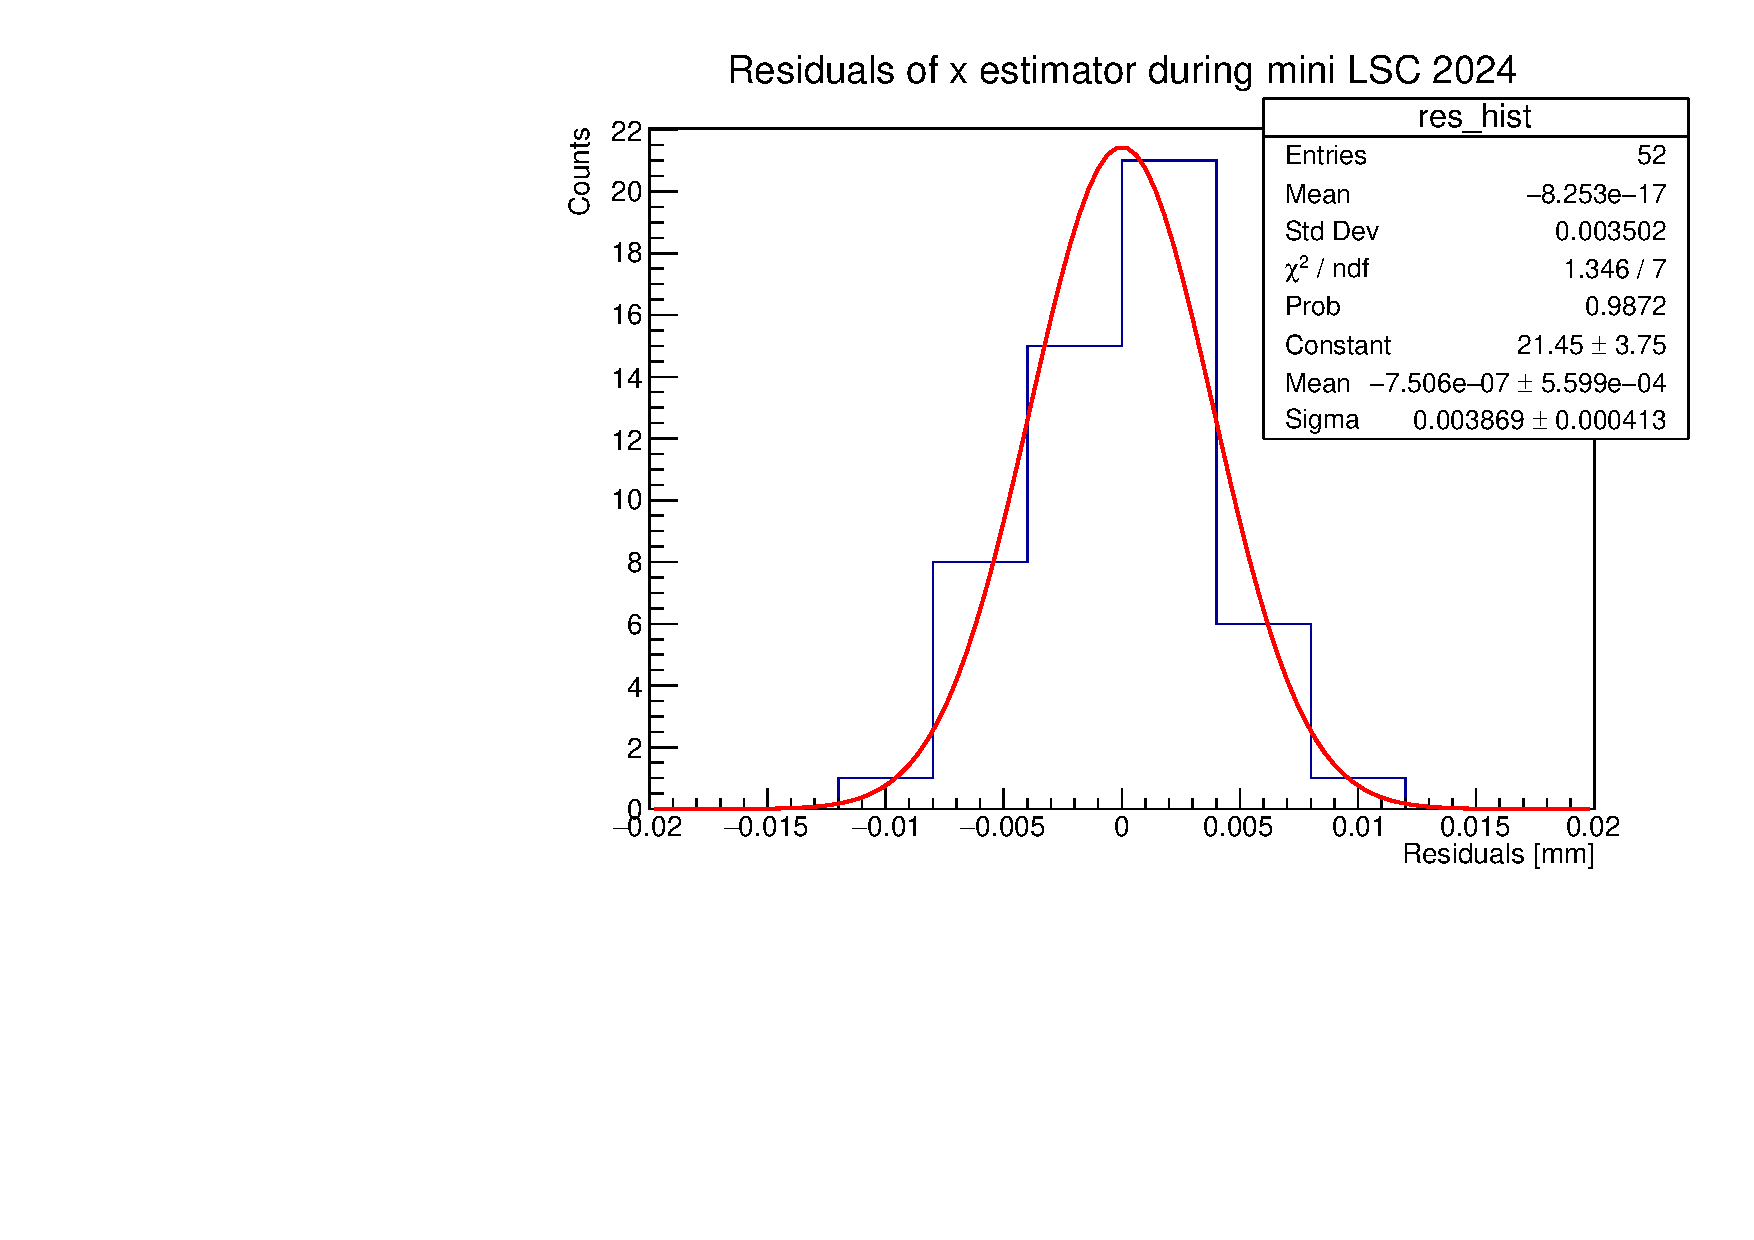
\includegraphics[width=\linewidth]{figures/x_fit_new.pdf}
    \caption{Residuals from the fit of the graph on the left. }\label{fig:xres_data}
    \end{subfigure}
    \caption{Linearity of the first component calculated with the PCA with respect to luminous beamline shifts in x component, alongside the residuals distribution fitted with a Gaussian distribution.}
    \label{fig:x_data}
\end{figure}


\begin{figure}
    \centering
    \begin{subfigure}{0.48\textwidth}
    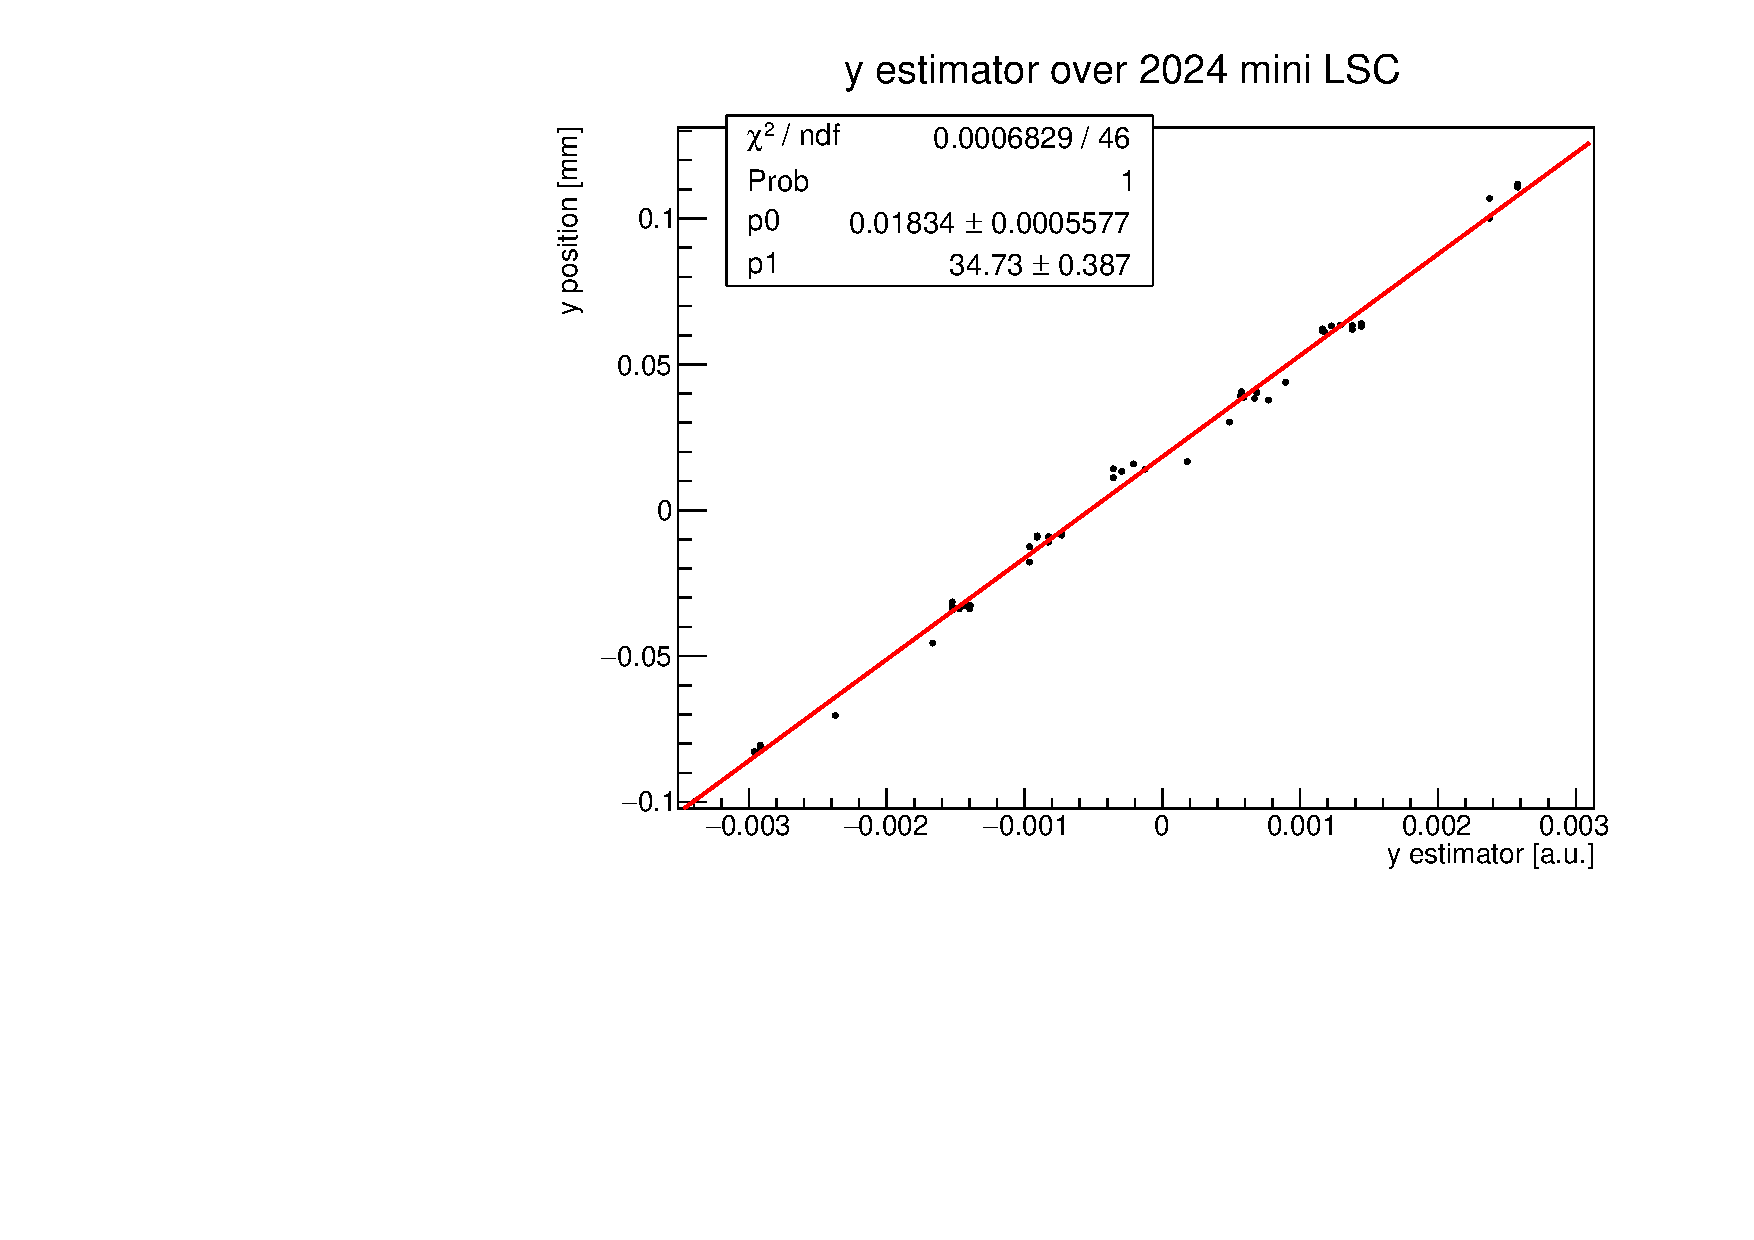
\includegraphics[width=\linewidth]{figures/y_fit_new.pdf}
    \caption{Linear Fit}\label{fig:yfit_data}
    \end{subfigure}
    \begin{subfigure}{0.48\textwidth}
    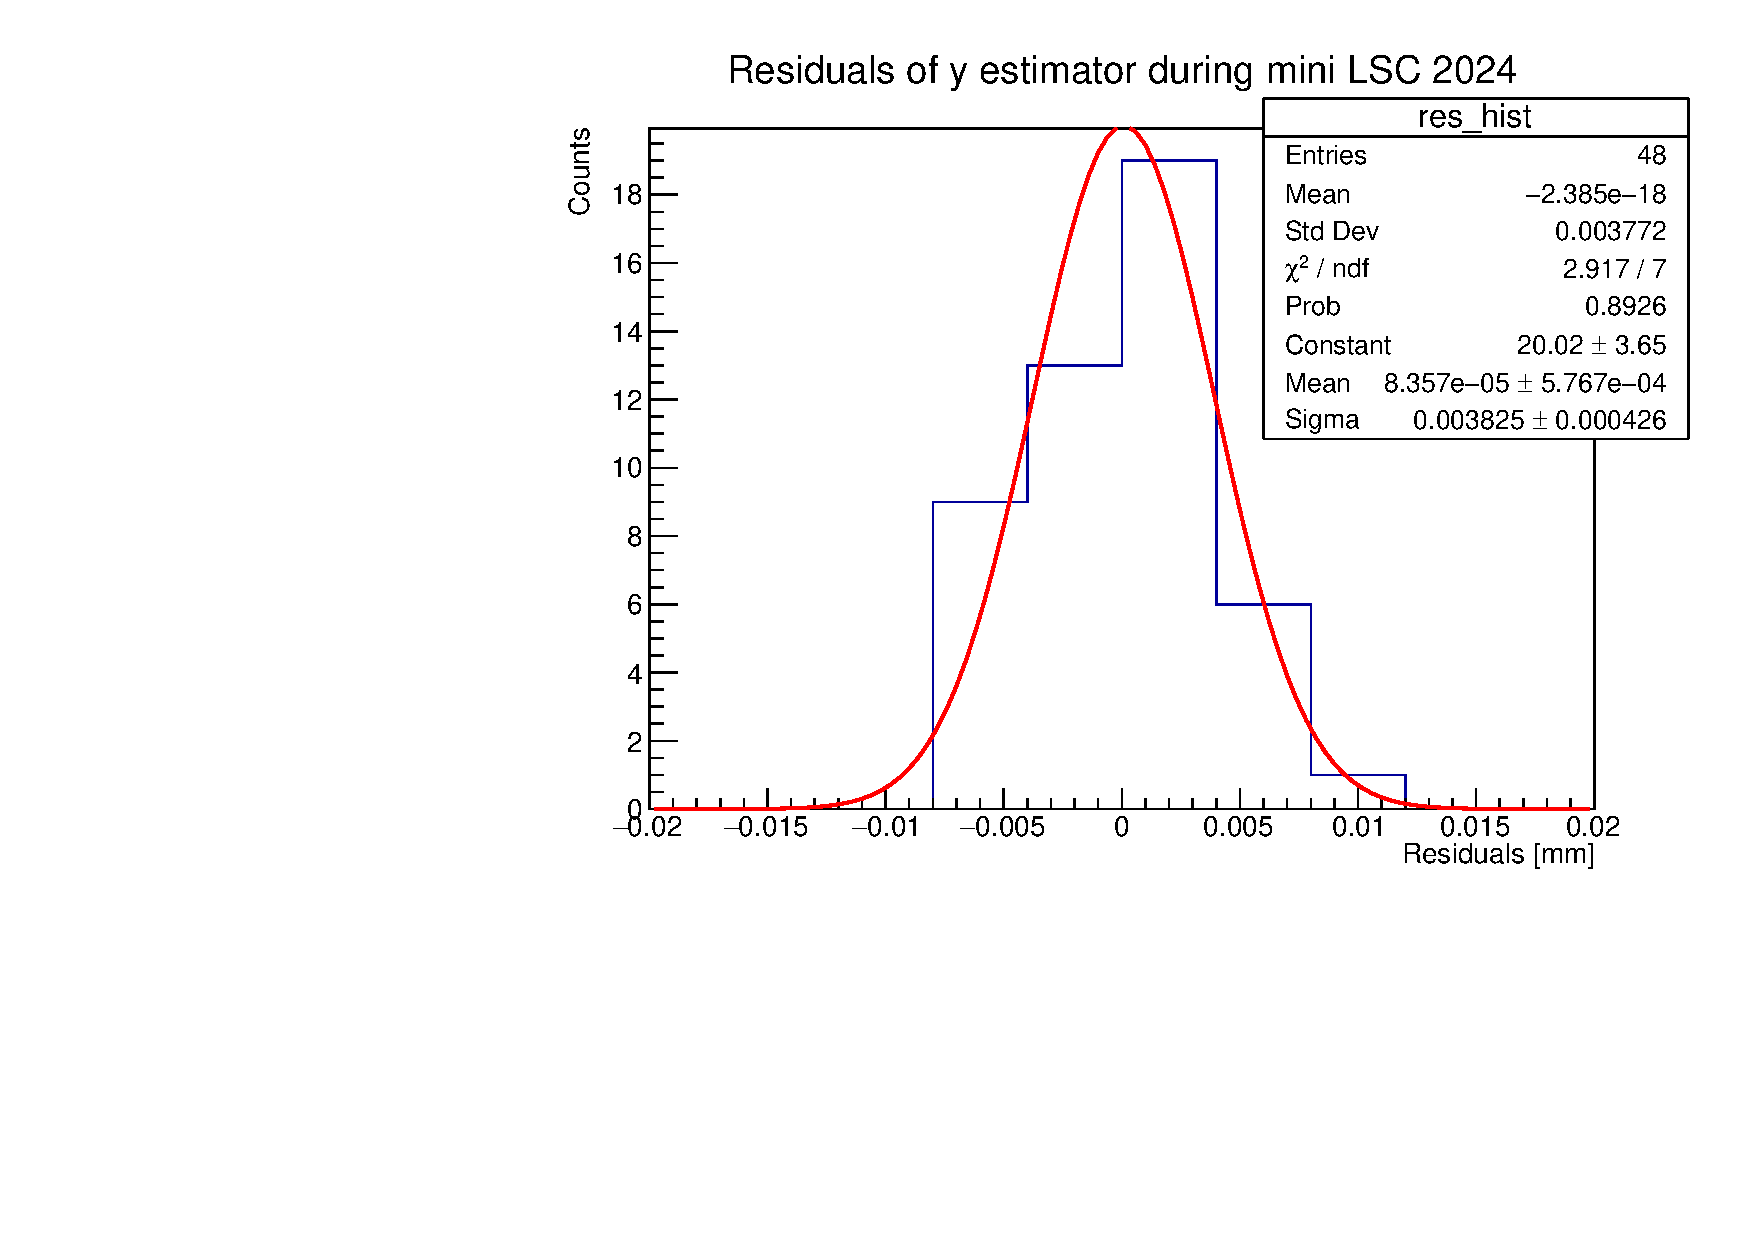
\includegraphics[width=\linewidth]{figures/y_res_new.pdf}
    \caption{Residuals from the fit of the graph on the left. }\label{fig:yres_data}
    \end{subfigure}
    \caption{Linearity of the first component calculated with the PCA with respect to beamline position shifts in y component, alongside the residuals distribution fitted with a Gaussian distribution.}
    \label{fig:y_data}
\end{figure}


The estimators $\hat{x}_{corrected}$ and $\hat{y}_{corrected}$ (green) are depicted as trending plots alongside with the mean set position of the beamline by LHC (orange), respectively in the first and second panel of Figure \ref{fig:traceplot_outliers}. As one can see, all the beamline shifts are followed quite smoothly, even the ones that were not used in the calibration. However there are two main issues:
\begin{itemize}
    \item there are some spikes at 13:38, 13:40 and 13:47. These spikes are due to saturation of the counters at restart of WinCC script or due to a change of Run. They do not represent a physical displacement of the beamline and therefore they must be treated.
    \item starting from 13:33 we have a first drop and then a displacement from the nominal position until the change of Run that happened around 13:47 for both $\hat{x}$ and $\hat{y}$ with respect to the set position. This could appear as a physical displacement of the beamline. However, by looking at the first panel of Figure \ref{fig:mini-vdm} we can see that around 13:33 a few counters dropped from their stable value. As one can see, the purple point indicate that at least one counter counted significantly less than the others. This behaviour is probably due to a drop in efficiency by specific counters. As soon as a Run is restarted (at 13:47), the efficiencies are restored to their nominal values and the correct behaviour of the counters is restored. We shall therefore discuss a robust method for handling this unexpected drops in efficiencies.
\end{itemize}

\begin{figure}
    \centering
    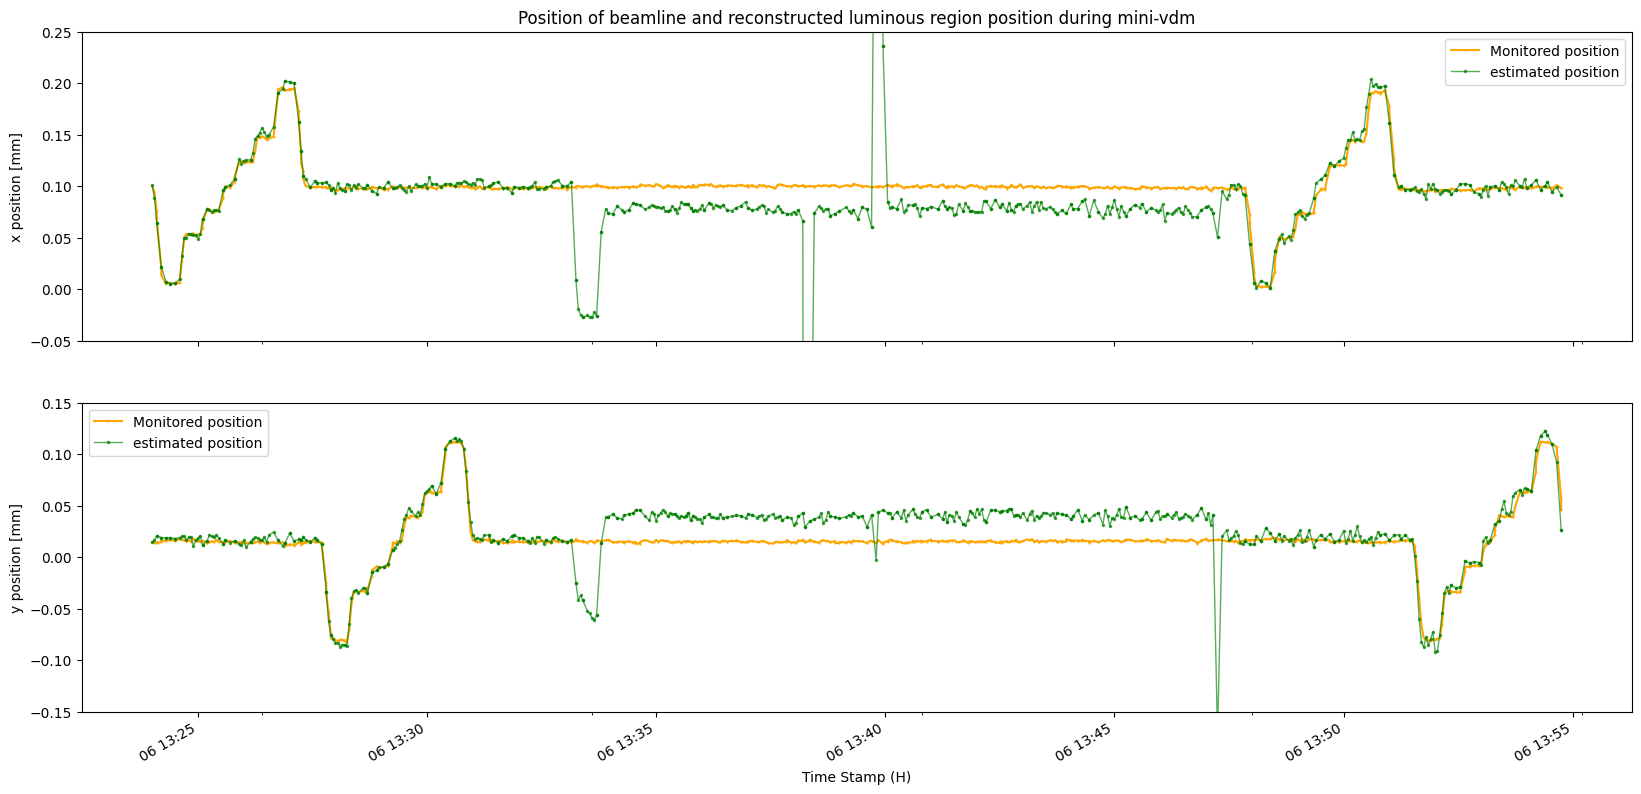
\includegraphics[width=\textwidth]{figures/traceplot_wo_median.png}
    \caption{Trending plot of the two estimators $\hat{x}_{corrected}$ and $\hat{y}_{corrected}$ (green), superimposed to the set position by LHC (orange).  }
    \label{fig:traceplot_outliers}
\end{figure}

To handle these anomalies and ensure robustness in data processing, we apply a filtering procedure to the cluster counter data at each timestamp. The steps are as follows:
\begin{itemize}
    \item Calculate the Medians: At each timestamp, we compute the median of all outer counters and the median of all inner counters separately and store them in a value $m_t$ differentiated based on the type $t$ outer or inner. This differentiation is needed because the average rate of the cluster changes according to their distance with respect to the beamline.
    \item Identify Outliers: Using the medians $m_t$ calculated in step 1, we identify outliers by checking if a counter value $c$ falls outside the interval $0.5 m_t < c < 1.5 m_t$ at each timestamp. Any counter whose value lies outside this range is considered an outlier.
    \item Replace Outlier Values: For counters identified as outliers, we replace their values with the median $m_t$ of the corresponding counter type $t$.
    \item Manage Spikes: To address sudden spikes in data, we apply a fixed threshold to the recorded counter value. If the recorded counter exceeds this threshold, we remove the entire reading for that timestamp, as these spikes typically indicate erroneous readings or other transient issues.
\end{itemize}

By implementing this filtering procedure, we produce a new traceplot with the new corrected estimators $\hat{x}_{median}$ and $\hat{y}_{median}$ in Figure \ref{fig:traceplot_off}. As one can see, both estimators overlap with the position reconstructed by the VELO monitoring tasks. 

\begin{figure}
    \centering
    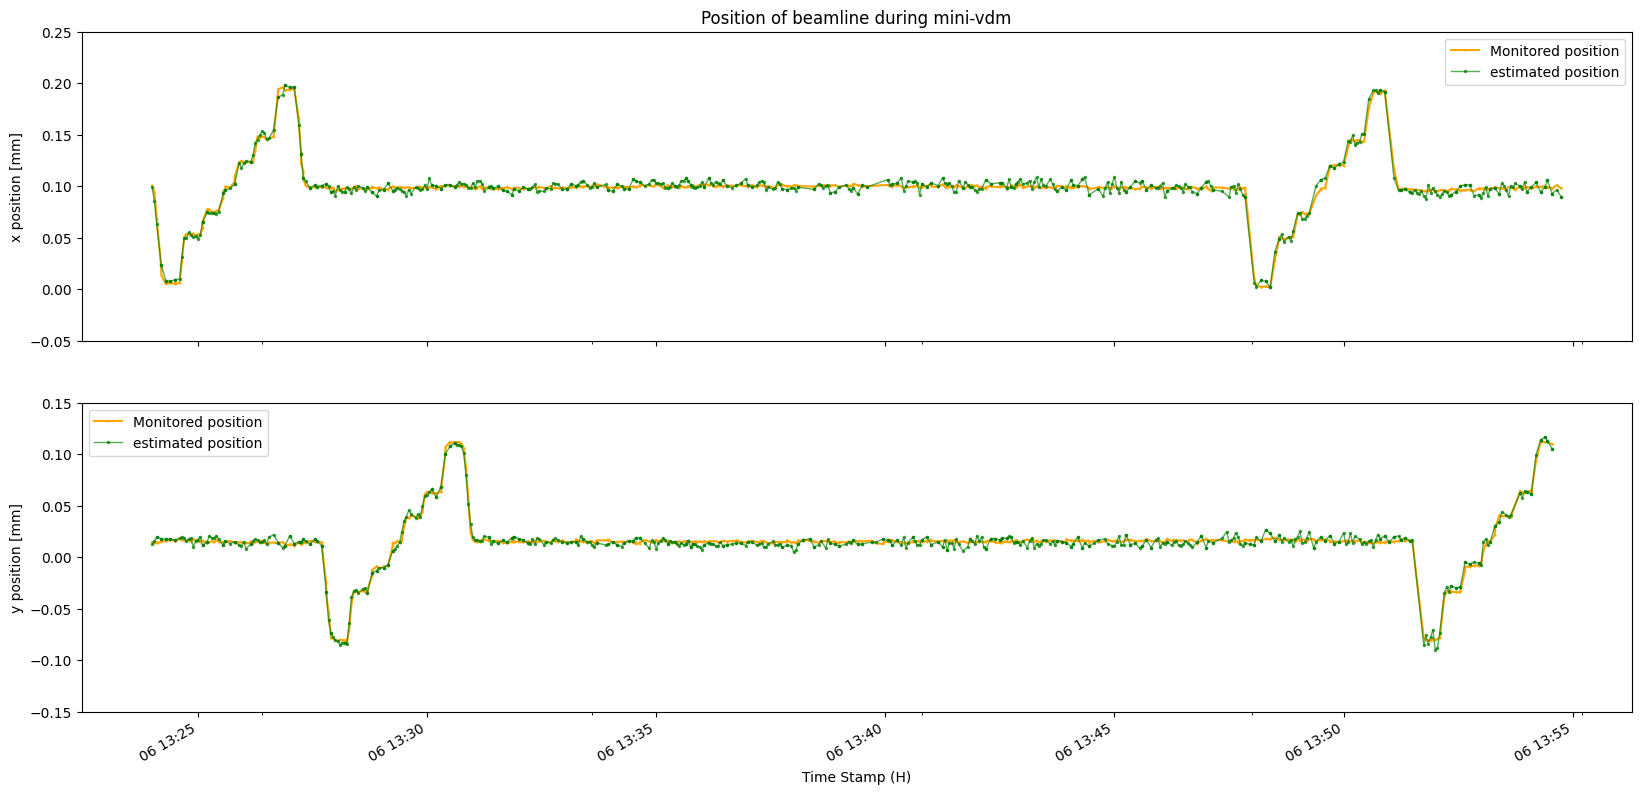
\includegraphics[width=\textwidth]{figures/traceplot_zoom.png}
    \caption{Trending plot of the two estimators $\hat{x}_{median}$ and $\hat{y}_{median}$ (green), superimposed to the reconstructed position of the transverse beamline position by the monitoring reconstruction tasks of the VELO (orange).}
    \label{fig:traceplot_off}
\end{figure}

A more quantitative analysis of the correctness of the estimated positions $\hat{x}_{median}$ and $\hat{y}_{median}$ can be performed by producing a scatter plot between the estimated positions $\hat{x}_{median}$, $\hat{y}_{median}$ vs the relative reconstructed positions by the monitoring tasks of the VELO during the whole Van der Meer fill. These scatter plot are available in Figures \ref{fig:xfit_comparison} and \ref{fig:yfit_comparison}, where we also performed a linear fit. If there is total accordance between these to quantities we expected the angular coefficients to be $p1=1$ and the offset $p0=0$ of the fitted line. 
The results of these fit are summarised in Table \ref{tab:summary}. All the estimated coefficients differ less than 2 $\sigma$ from their expected value. 


\begin{figure}
    \centering
    \begin{subfigure}{0.48\textwidth}
    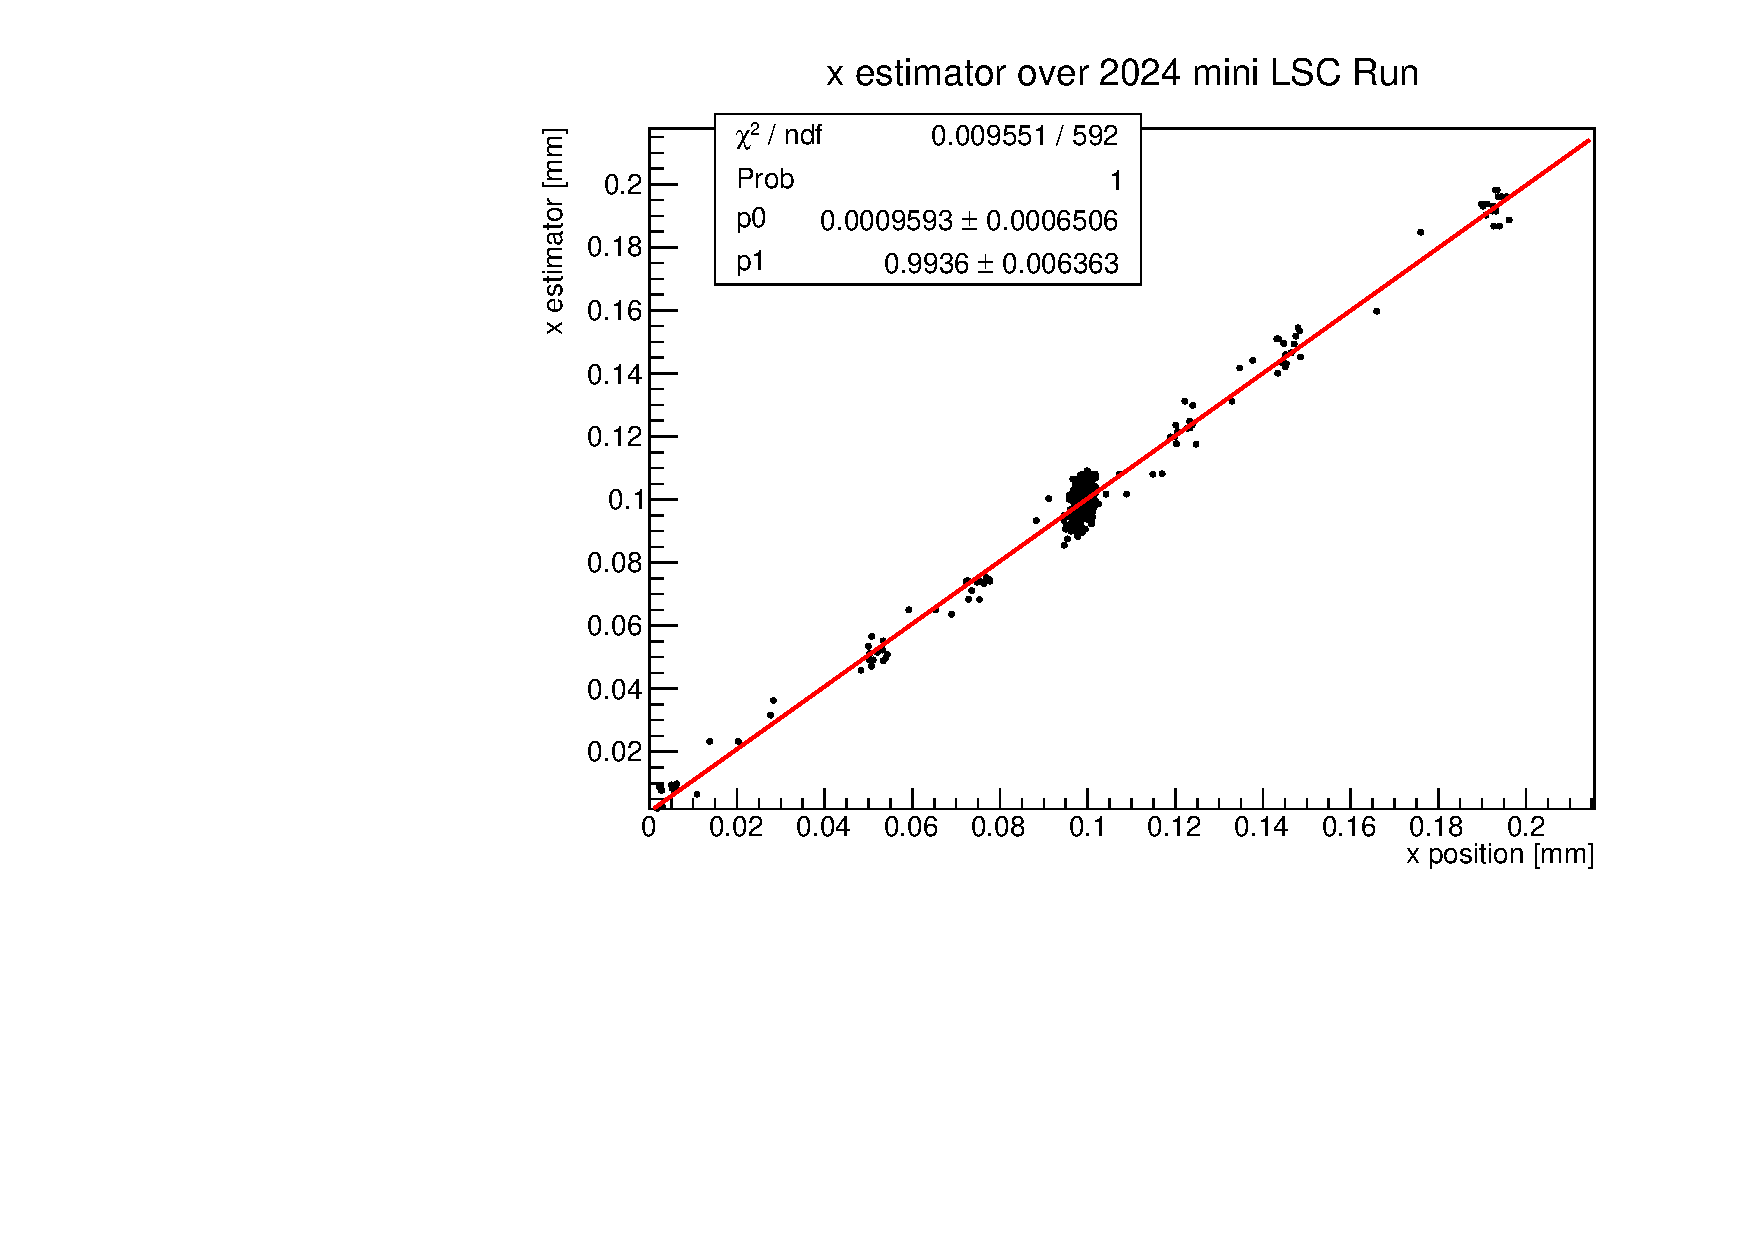
\includegraphics[width=\linewidth]{figures/x_comparison_side.pdf}
    \caption{Linear Fit}\label{fig:xfit_comparison}
    \end{subfigure}
    \begin{subfigure}{0.48\textwidth}
    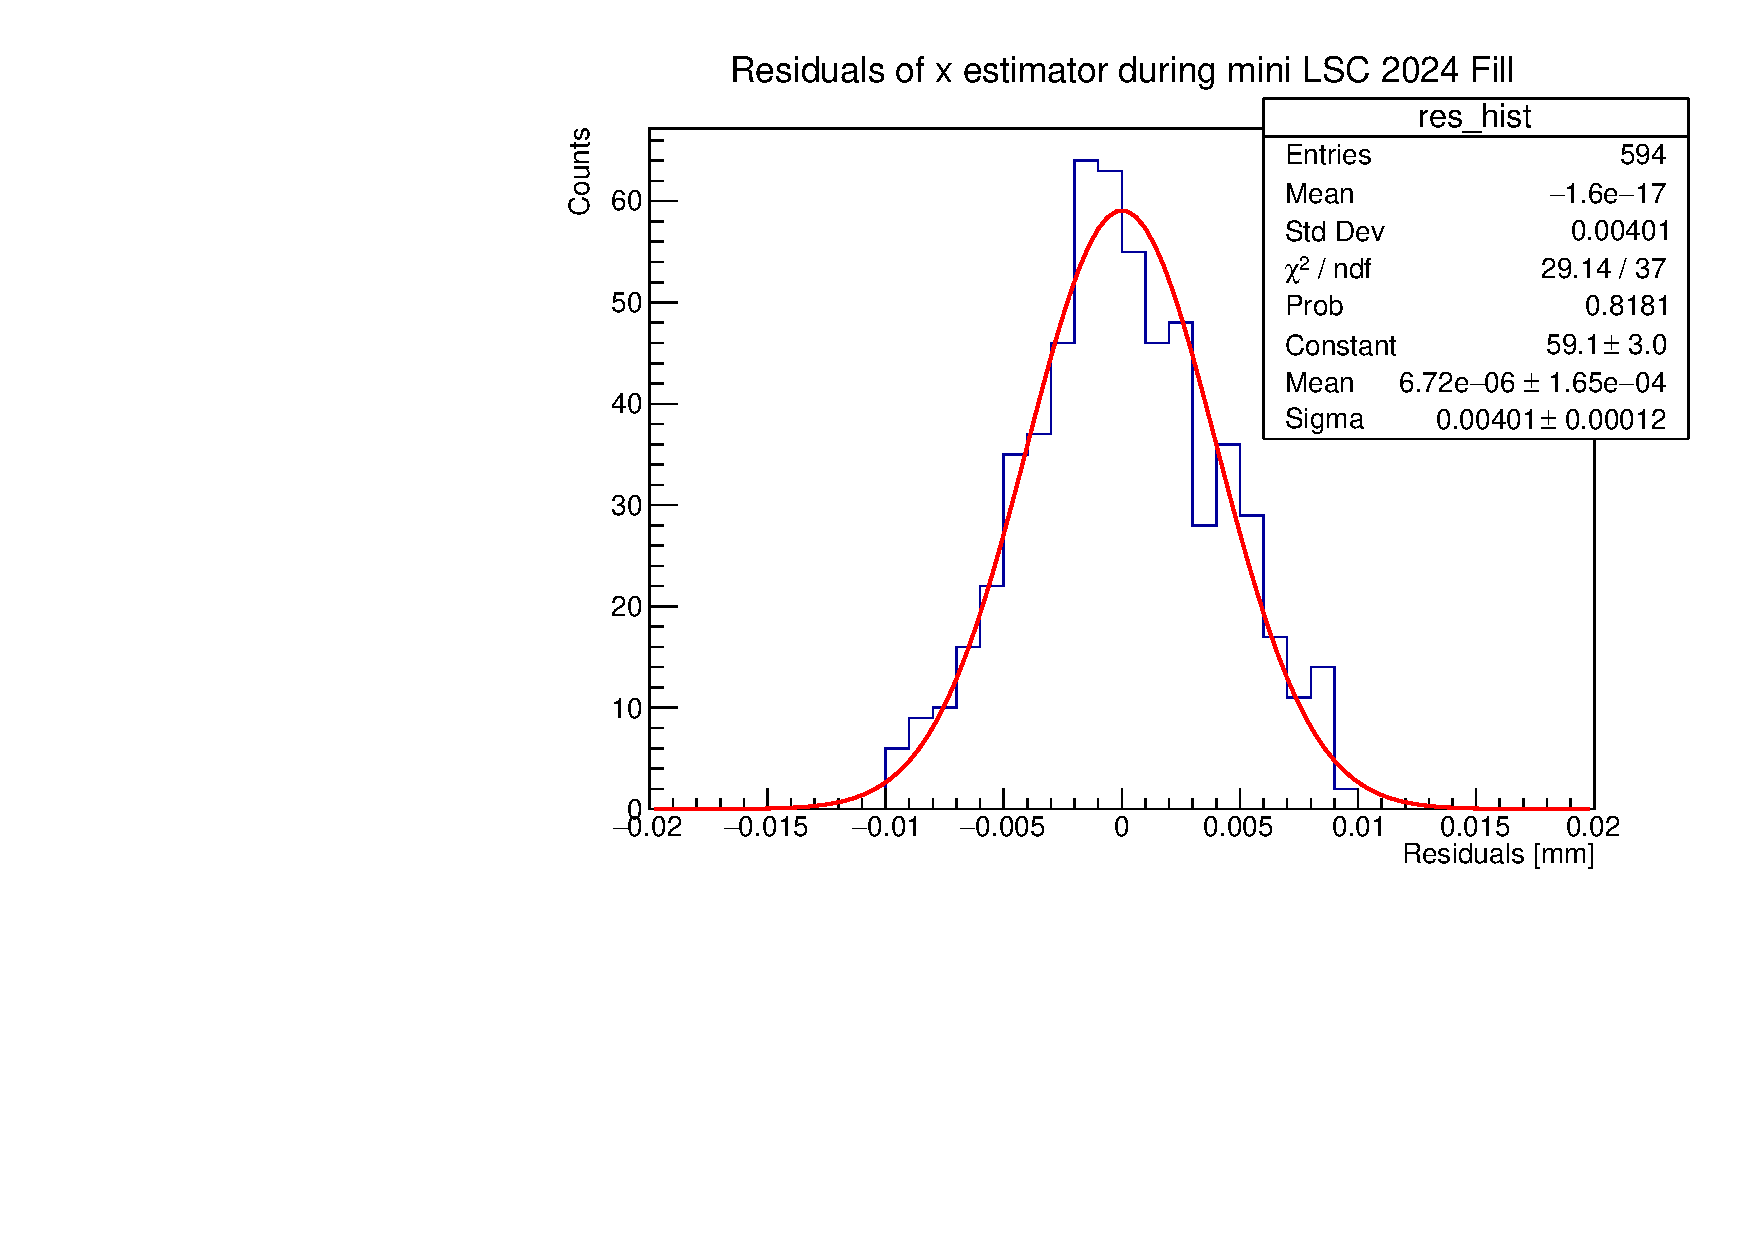
\includegraphics[width=\linewidth]{figures/x_comparison_res_side.pdf}
    \caption{Residuals from the fit of the graph on the left. }\label{fig:xres_comparison}
    \end{subfigure}
    \caption{$\hat{x}_{median}$ estimator vs beamline position shifts in x component, alongside the residuals distribution fitted with a Gaussian distribution.}
    \label{fig:x_comaprison}
\end{figure}



\begin{figure}
    \centering
    \begin{subfigure}{0.48\textwidth}
    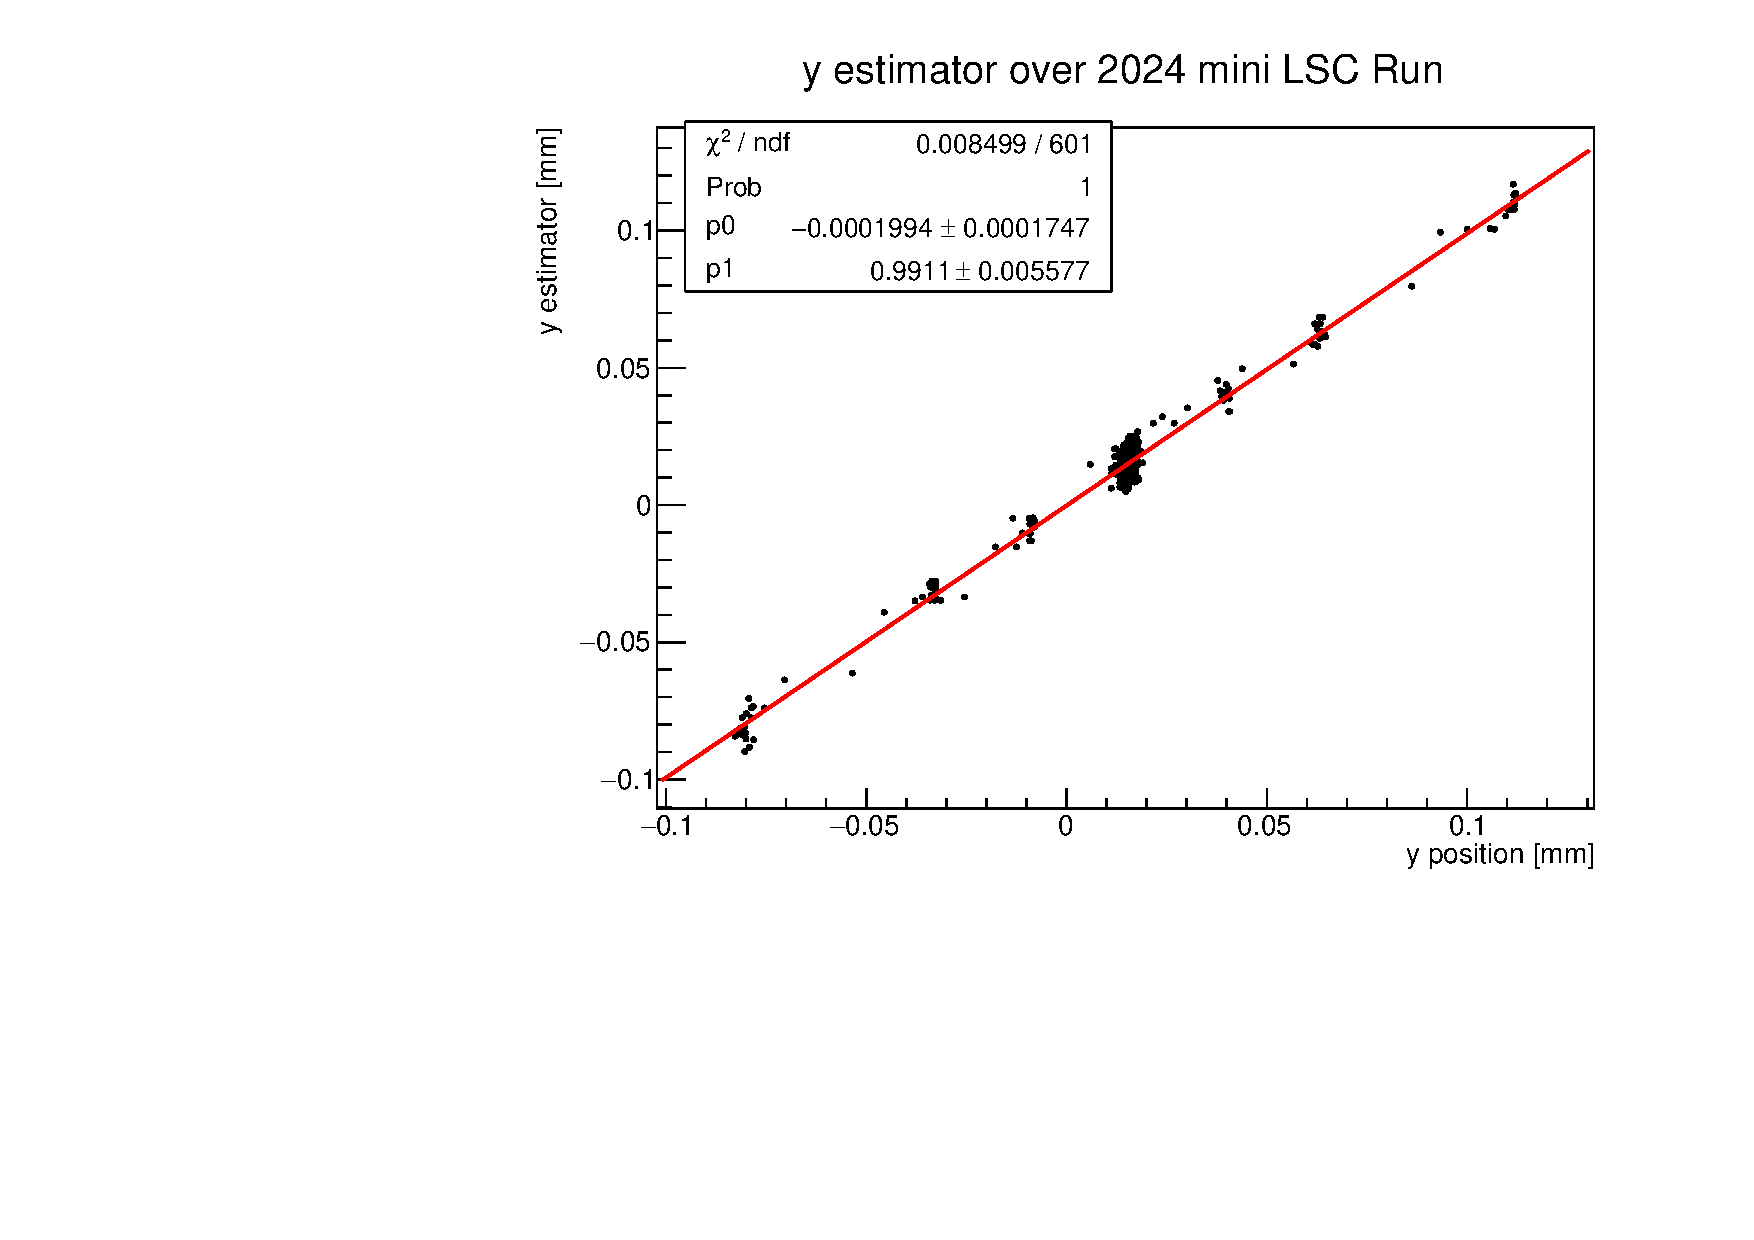
\includegraphics[width=\linewidth]{figures/y_comparison_side.pdf}
    \caption{Linear Fit}\label{fig:yfit_comparison}
    \end{subfigure}
    \begin{subfigure}{0.48\textwidth}
    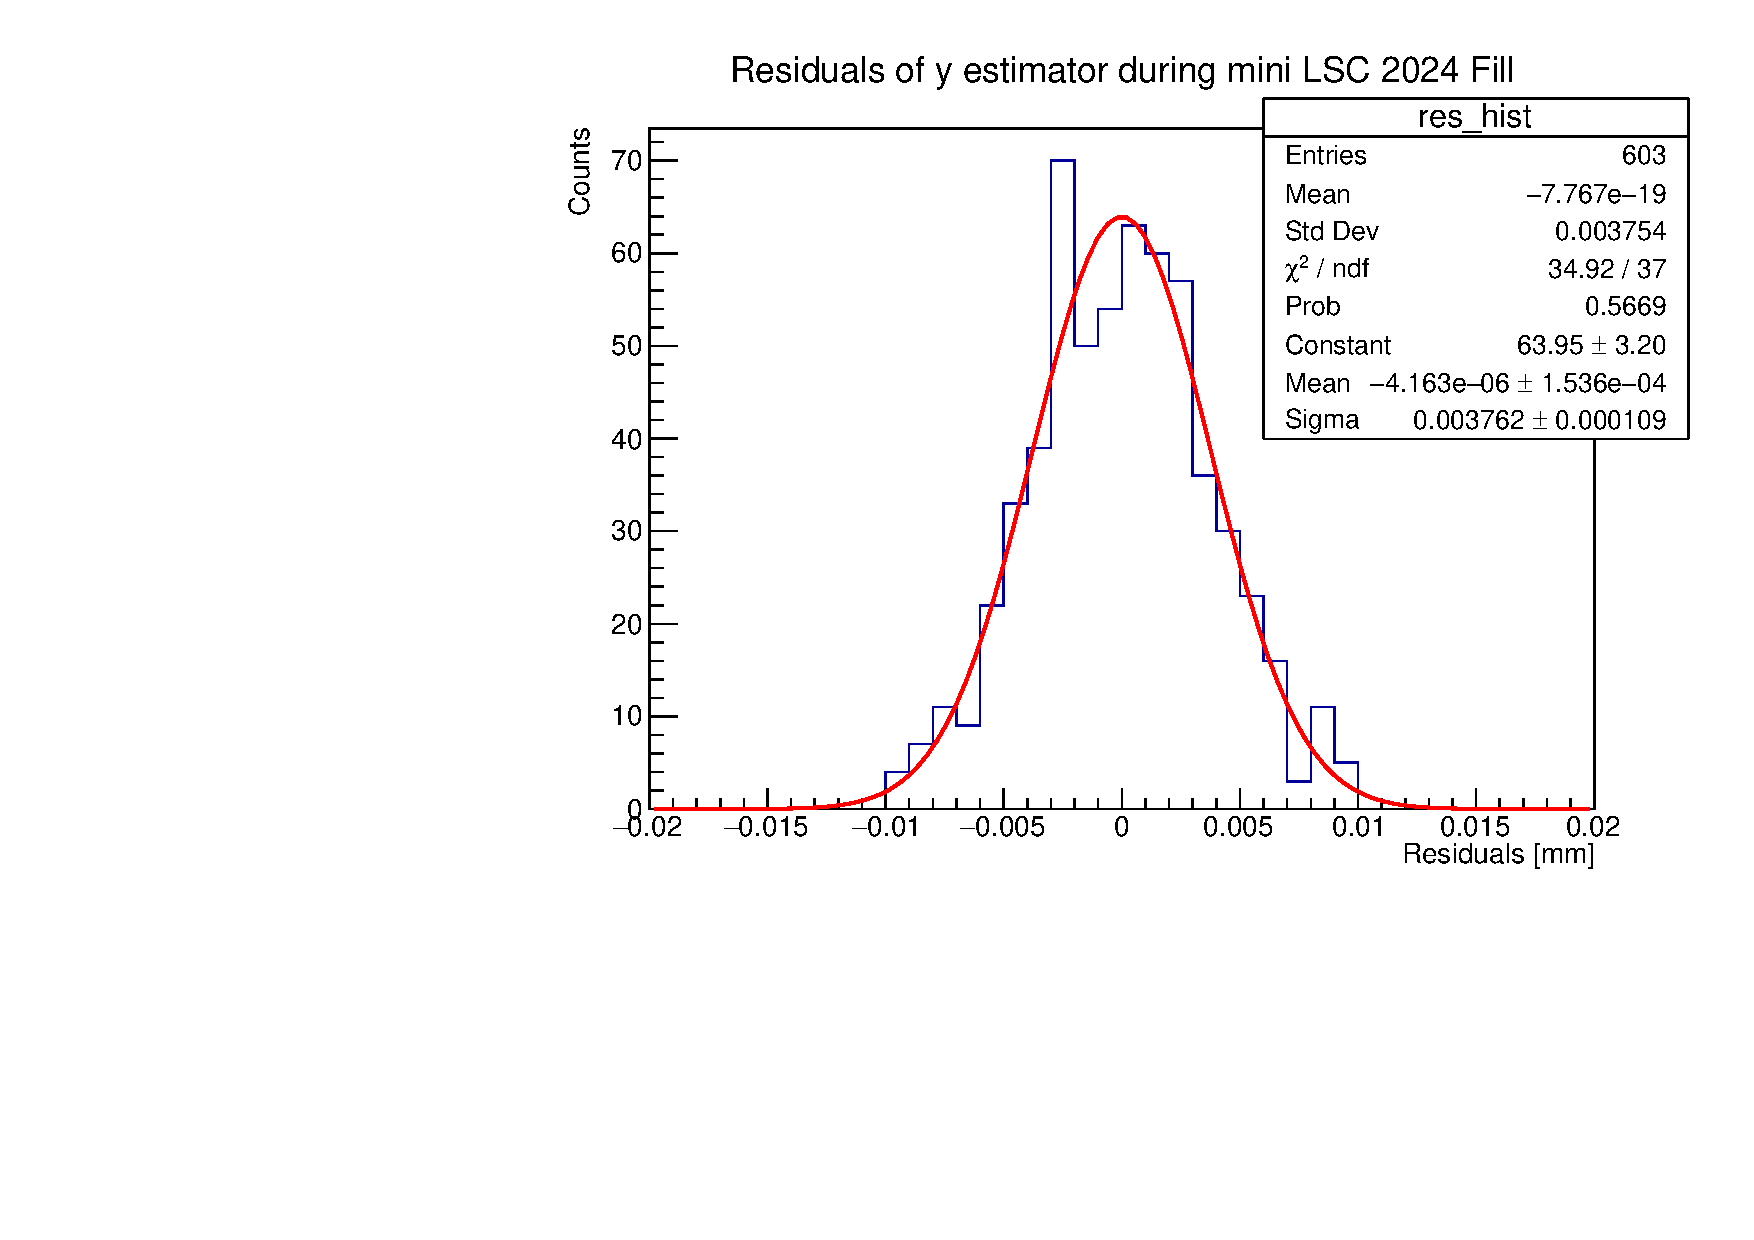
\includegraphics[width=\linewidth]{figures/y_comparison_res_side.pdf}
    \caption{Residuals from the fit of the graph on the left. }\label{fig:yres_comparison}
    \end{subfigure}
    \caption{$\hat{y}_{median}$ estimator vs beamline position shifts in y component, alongside the residuals distribution fitted with a Gaussian distribution.}
    \label{fig:y_comparison}
\end{figure}

\begin{table}
    \centering
    \begin{tabular}{c|c|c|c|c|c|c}
    variable  & $p0$ & $p1$ & $\sigma_{p0}$ & $\sigma_{p1}$ & distance $p0=0$ [$\sigma$] & distance $p1=1$ [$\sigma$]\\
    \hline
       x  & 0.00096 & 0.9936 & 0.00065 & 0.0064 & 1.5 & 1\\
       y  & -0.00020 & 0.9911 & 0.00017 & 0.0056 & 1.2 & 1.6 
    \end{tabular}
    \caption{Summary of comparison between estimators and monitored positions by the VELO}
    \label{tab:summary}
\end{table}

In the Figures \ref{fig:xres_comparison} and \ref{fig:yres_comparison} we report an histogram of the residuals from the fitted function, alongside with a Gaussian fit. From the Sigma of the fitted Gaussian we can quote a resolutions of the two estimators $\hat{x}$ and $\hat{y}$, which is quoted to be $\SI{4}{\micro\meter}$.

Considering that in the VdM conditions of April 6th 2024 there were 8 bunches in collisions, this correspond to an approximate trigger rate of $\SI{88}{\kilo\hertz}$, assuming that the trigger was performed on each colliding bunch. For a readout every 3 seconds, the counters integrate 264000 events but at a nominal $\mu=8.5$, much higher than the one used for Run~3 physics condition $\mu=5.5$. The higher number of PVs in this Fill takes us to define a number of ``equivalent events", which are the number of events that at a $\mu=5.5$ would contain the same number of PVs observed in this Fill at $\mu=8.5$. Since the number of PVs scale linearly with $\mu$, in this fill we have a number of equivalent integrated events equal to$N_{data}=264000\tfrac{8.5}{5.5}=408000$. This number of ``equivalent events" is useful in order to compare the resolution quoted for the data to the one estimated in the MC. In fact, in the data we integrate much more statistics than the one in the MC, corresponding to a factor $\tfrac{408000}{20000}=20.4$.  The increase in the statistics is responsible for a more accurate estimation of the counters rate $\mathbf{\lambda}$ that are used for the estimation of the scores $\mathbf{t}_{1}$. Assuming that only the counter rates contribute to the uncertainty, we expected that the resolution quoted for the estimators in the MC is a factor $\sqrt{20.4}$ worse than the one we reported in Figures \ref{fig:xres_comparison} and \ref{fig:yres_comparison} for the MC. In fact, calculating
\begin{equation}
    \sigma_{MC}^{expected} = \sigma_{data}\sqrt{20.4} \approx \SI{18}{\micro\meter},
\end{equation}
which approximately corresponds to the value $\SI{20}{\micro\meter}$ reported in the Figures  \ref{fig:xres_MC} and \ref{fig:yres_MC}. This calculation make use only of the statistical uncertainty given by the mean of the counters per event, so we expect it to be underestimated. Other factors (i.e the uncertainties on the weights $\mathbf{w_{(1)}}$) and approximations could be responsible for the $\SI{5}{\micro\meter}$ difference that we observe in Figures  \ref{fig:xres_MC} and \ref{fig:yres_MC}. However, getting an estimate of the same order of magnitude is a reassuring result.

Regarding the $z$ variable, during this fill its value was maintained constant, therefore it was not possible to calibrate it. It is intended to extract the information of the true PVs from a whole physics fill and perform the calibration directly on this physics fill. Unfortunately, we were not able to perform this calibration before the conclusion of this thesis work. 


%recap sull'algoritmo finale
\section{Deployment in the LHCb online system}\label{sec:beamline_integration}
The estimated luminous region can be integrated into the online monitoring system. In order to construct these estimators we need to leverage the information provided by each counter position in different VELO modules. The ASICs that read each VELO module send the data via optical fibres to the TELL40s board, where the clustering algorithm is performed. As presented in Section \ref{sec:ecs}, ECS has access to the all the TELL40s simultaneously, therefore it is the most suitable environment for performing the combination of the cluster counters with the weight vectors in order to get the luminous region position estimators. By integrating in the WinCC project that handles ECS a WinCC script that compute the various estimators, we can get \textit{datapoints} that allows a monitoring in real time.
In order to summarise what was exposed in this chapter and the various corrections performed on the form of the estimators presented in \eqref{x_hat_true}, we report the Algorithm \ref{alg:beamline} used to compute the luminous region position that operates online. This algorithm is rather conceptional than operational, since the actual script that runs online is written using built-in function and optimised in order to perform the minimal number of possible for loops. %However, this formulation reports all the important passages needed to compute the beamline estimation.

\begin{algorithm}
\caption{Beamline Position Estimation}\label{alg:beamline}
\begin{algorithmic}[1]
\ENSURE  INT poolPeriod = 3 seconds.
\ENSURE  FLOAT $w_x$[208]: weights for x estimate
\ENSURE  FLOAT $w_y$[208]: weights for y estimate
\ENSURE  FLOAT $a_x$,$ b_x$, $a_y$, $b_y$: coefficients for calibration 
\WHILE{true}
    \IF{(current time modulo poolPeriod) == 0}
        \STATE FLOAT  bb[208]: Get 208 cluster counters of type bb and store it in array.
        \STATE FLOAT  be[208]: Get 208 cluster counters of type be and store it in array.
        \STATE FLOAT  eb[208]: Get 208 cluster counters of type eb and store it in array.
        \STATE FLOAT  ee[208]: Get 208 cluster counters of type ee and store it in array.
        \STATE FLOAT c[208]: empty array that will host counters without background.
        \STATE FLOAT MU: Get $\mu$ value.
        \FOR{i=0 \TO 208 } 
        \IF{0 < bb[i], be[i], eb[i], ee[i] < 10}
        \STATE {c[i] =  bb[i] -  be[i] -  eb[i] +  ee[i]}     
        \ELSE
        \STATE c[i] = BADREAD
        \ENDIF
        \ENDFOR
        \STATE Compute median of the counters differentiated by data type excluding BADREAD 
        \STATE FLOAT x,y=0
        \FOR{i=0 \TO 208}
        \IF{(c[i] == BADREAD \OR c[i] < 0.5 * median type \OR c[i] > 1.5 * median type)}
            \STATE c[i] = median type 
        \ENDIF
        \STATE x= x+ c[i]*$w_x$[i]
        \STATE y= x+ c[i]*$w_y$[i]
        \ENDFOR
        \STATE x= $a_x$* x/MU + $b_x$
        \STATE y= $a_y$ * y/MU +$b_y$
        \IF{all c[i] != BADREAD}
        \STATE write x, y in register
        \ENDIF
    \ENDIF
\ENDWHILE
\end{algorithmic}
\end{algorithm}


Once the luminous region position \textit{datapoints} are stored, we can also plot them using the LHCb official tool for the online monitoring, i.e. \textit{Monet}. We created a web-page containing the trending plot of the luminous region position in the both $x$ and $y$ component as a function of the local time.

\begin{figure}
    \centering
    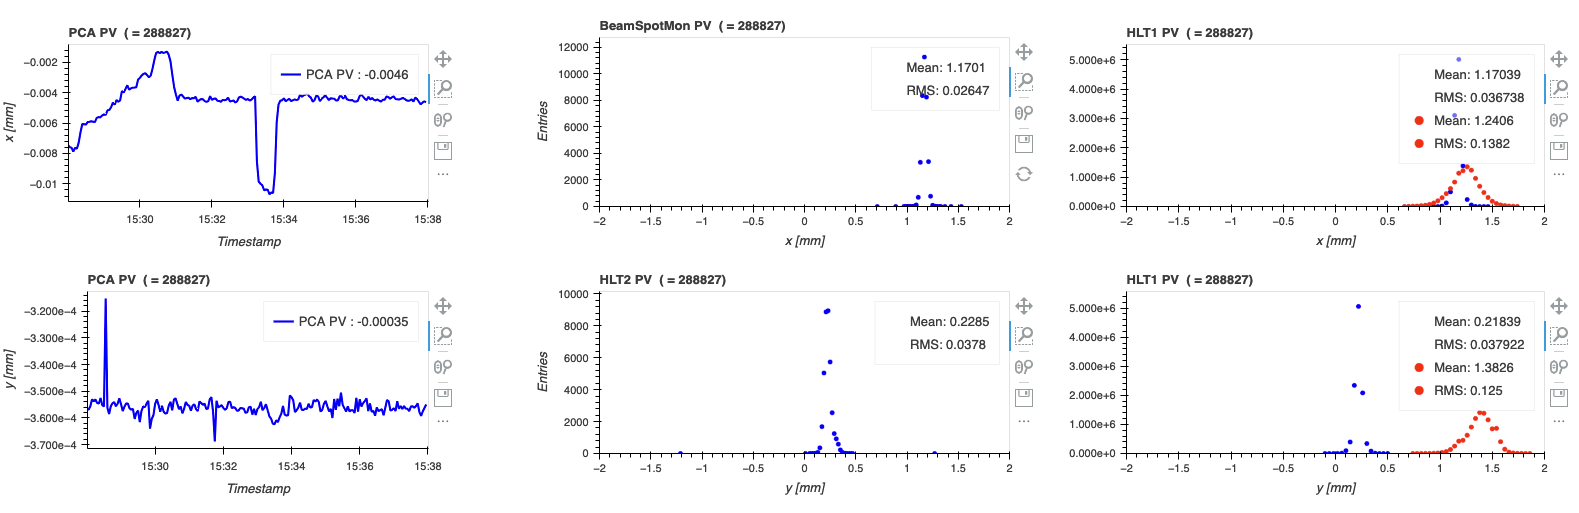
\includegraphics[width=\textwidth]{figures/Monet_beamline_screen.png}
    \caption{Screenshot of the Monet web-page during the LSC fill of April 6th 2024. The two components of the luminous region position are presented on the left, while on the centre we reported the positions calculated by BeamSpotMonitor. On the right the mean PVs calculated by HLT$1$ with different alignment constants (red and blue)}
    \label{fig:monet_beamline}
\end{figure}

In Figure \ref{fig:monet_beamline} a screenshot of the early implementation of this web-page is reported, where we report our estimators (left), alongside the reconstructed position by BeamSpotMonitor (centre) and the reconstructed PVs by HLT$1$ (right), with the red and blue points of the latter corresponding to different alignments constants. The screenshot was taken during the LSC of April 6th 2024. In this early implementation the various corrections for outliers and missing counters were still not implemented, explaining the strange drop at 15:33 we also see in Figure~\ref{fig:traceplot_outliers}\footnote{The online plot is shifted because all the analysis presented in the chapter were performed using UCT time, therefore two hours backwards shifted with respect to local Geneva time.}. Furthermore, in this implementation the estimators were not calibrated and the two components were swapped. Although uncalibrated and uncorrected, in the upper left panel we appreciate the ramp of LSC, proving the sensitivity of the estimators and the correct online deployment.
A further development of this web-page will be described in Section \ref{sec:integration_detector}, as we will include other parameters in the left plots.

The next step in the integration into the LHCb system can take two paths: either the information of the luminous region position is stored in the raw banks to use for offline analysis or the position is given as input to the PVs reconstruction algorithms that runs at HLT$1$. As this thesis is being written, it is still under investigation which one of these options is to prefer.